\pdfminorversion=4
\documentclass{beamer}

\usepackage{tikz}
\usepackage[toc]{beamerthemecea2019}
\usepackage[T1]{fontenc}
\usepackage[utf8]{inputenc}

\usepackage{longtable}
%\usepackage{couleurs}
\usepackage{listings}
%\usepackage{mecanique}
\usepackage{pifont}% http://ctan.org/pkg/pifont
\usepackage{animate,subcaption}
\usepackage[absolute,overlay]{textpos}
\setlength{\TPHorizModule}{\paperwidth}
\setlength{\TPVertModule}{\paperheight}

\newcommand{\backupbegin}{
   \newcounter{finalframe}
   \setcounter{finalframe}{\value{framenumber}}
}
\newcommand{\backupend}{
   \setcounter{framenumber}{\value{finalframe}}
}
\setbeamercolor{block title}{bg=cea_rouge!90,fg=white}
\newcommand{\dx}{\text{ dx}}
\newcommand{\dS}{\text{ dS}}
\newcommand{\udl}[1]{\boldsymbol{#1}}
\newcommand{\uddl}[1]{\boldsymbol{#1}}
\renewcommand{\div}{\operatorname{div}}
\newcommand{\bg}{\boldsymbol{g}}
\newcommand{\bj}{\boldsymbol{j}}
\newcommand{\bu}{\boldsymbol{u}}
\newcommand{\bv}{\boldsymbol{v}}
\newcommand{\bvarepsilon}{\boldsymbol{\varepsilon}}
\newcommand{\bsig}{\boldsymbol{\sigma}}
\newcommand{\bD}{\boldsymbol{D}}
\newcommand{\bE}{\boldsymbol{E}}
\newcommand{\bF}{\boldsymbol{F}}
\newcommand{\bR}{\boldsymbol{R}}
\newcommand{\bH}{\boldsymbol{H}}
\newcommand{\bI}{\boldsymbol{I}}
\newcommand{\bP}{\boldsymbol{P}}
\newcommand{\bS}{\boldsymbol{S}}
\newcommand{\bT}{\boldsymbol{T}}
\newcommand{\bV}{\boldsymbol{V}}
\newcommand{\bY}{\boldsymbol{Y}}
\newcommand{\Bb}{\mathcal{B}}
\newcommand{\Dd}{\mathcal{D}}
\newcommand{\Ee}{\mathcal{E}}
\newcommand{\CC}{\mathbb{C}}
\newcommand{\DD}{\mathbb{D}}
\newcommand{\TT}{\mathbb{T}}
\newcommand{\Sig}{\boldsymbol{\Sigma}}
\newcommand{\T}{^\text{T}}
\newcommand{\jump}[1]{[\![#1]\!]}
\DeclareMathOperator*{\argmin}{arg\,min}
\DeclareMathOperator{\tr}{tr}
\newcommand{\pavg}[1]{\left\langle #1 \right\rangle}

\newcommand{\Cxx}{\texttt{C\nolinebreak\hspace{-.05em}\raisebox{.4ex}{\tiny\bf +}\nolinebreak\hspace{-.10em}\raisebox{.4ex}{\tiny\bf +}}
  \def\CC{{C\nolinebreak[4]\hspace{-.05em}\raisebox{.4ex}{\tiny\bf ++}}}}
\newcommand{\tfel}{\href{http://www.tfel.sourceforge.net}{\texttt{TFEL}}}
\newcommand{\mfront}{\href{http://www.tfel.sourceforge.net}{\texttt{MFront}}}
\newcommand{\cea}{\href{http://www.cea.fr}{CEA}}
\newcommand{\edf}{\href{http://www.edf.com}{EDF}}
\newcommand{\inria}{\href{http://www.inria.fr}{INRIA}}
\newcommand{\gcc}{\href{https://gcc.gnu.org/}{gcc}}
\newcommand{\clang}{\href{clang.llvm.org}{clang}}
\newcommand{\icc}{\href{https://software.intel.com/en-us/c-compilers}{icc}}
\newcommand{\msys}{\href{http://www.mingw.org/wiki/MSYS}{MSYS}}
\newcommand{\jenkins}{\href{http://jenkins-ci.org}{\texttt{Jenkins}}}
\newcommand{\gpl}{\href{http://www.gnu.org/licenses/gpl-3.0.txt}{GNU Public License}}
\newcommand{\unix}{\texttt{Unix}}
\newcommand{\linux}{\texttt{LiNuX}}
\newcommand{\freebsd}{\href{https://www.freebsd.org/}{\texttt{FreeBSD}}}
\newcommand{\opensolaris}{\texttt{OpenSolaris}}
\newcommand{\cygwin}{\texttt{cygwin}}
\newcommand{\wsl}{\texttt{Windows Subsystem for LiNuX}}
\newcommand{\haiku}{\texttt{Haiku}}
\newcommand{\mtest}{\texttt{mtest}}
\newcommand{\absvalue}[1]{{\left|#1\right|}}

\usepackage{fancyvrb}
\newcommand{\VerbBar}{|}
\newcommand{\VERB}{\Verb[commandchars=\\\{\}]}
\DefineVerbatimEnvironment{Highlighting}{Verbatim}{commandchars=\\\{\}}
\newenvironment{Shaded}{}{}
\newcommand{\AlertTok}[1]{\textcolor[rgb]{1.00,0.00,0.00}{\textbf{#1}}}
\newcommand{\AnnotationTok}[1]{\textcolor[rgb]{0.38,0.63,0.69}{\textbf{\textit{#1}}}}
\newcommand{\AttributeTok}[1]{\textcolor[rgb]{0.49,0.56,0.16}{#1}}
\newcommand{\BaseNTok}[1]{\textcolor[rgb]{0.25,0.63,0.44}{#1}}
\newcommand{\BuiltInTok}[1]{#1}
\newcommand{\CharTok}[1]{\textcolor[rgb]{0.25,0.44,0.63}{#1}}
\newcommand{\CommentTok}[1]{\textcolor[rgb]{0.38,0.63,0.69}{\textit{#1}}}
\newcommand{\CommentVarTok}[1]{\textcolor[rgb]{0.38,0.63,0.69}{\textbf{\textit{#1}}}}
\newcommand{\ConstantTok}[1]{\textcolor[rgb]{0.53,0.00,0.00}{#1}}
\newcommand{\ControlFlowTok}[1]{\textcolor[rgb]{0.00,0.44,0.13}{\textbf{#1}}}
\newcommand{\DataTypeTok}[1]{\textcolor[rgb]{0.56,0.13,0.00}{#1}}
\newcommand{\DecValTok}[1]{\textcolor[rgb]{0.25,0.63,0.44}{#1}}
\newcommand{\DocumentationTok}[1]{\textcolor[rgb]{0.73,0.13,0.13}{\textit{#1}}}
\newcommand{\ErrorTok}[1]{\textcolor[rgb]{1.00,0.00,0.00}{\textbf{#1}}}
\newcommand{\ExtensionTok}[1]{#1}
\newcommand{\FloatTok}[1]{\textcolor[rgb]{0.25,0.63,0.44}{#1}}
\newcommand{\FunctionTok}[1]{\textcolor[rgb]{0.02,0.16,0.49}{#1}}
\newcommand{\ImportTok}[1]{#1}
\newcommand{\InformationTok}[1]{\textcolor[rgb]{0.38,0.63,0.69}{\textbf{\textit{#1}}}}
\newcommand{\KeywordTok}[1]{\textcolor[rgb]{0.00,0.44,0.13}{\textbf{#1}}}
\newcommand{\NormalTok}[1]{#1}
\newcommand{\OperatorTok}[1]{\textcolor[rgb]{0.40,0.40,0.40}{#1}}
\newcommand{\OtherTok}[1]{\textcolor[rgb]{0.00,0.44,0.13}{#1}}
\newcommand{\PreprocessorTok}[1]{\textcolor[rgb]{0.74,0.48,0.00}{#1}}
\newcommand{\RegionMarkerTok}[1]{#1}
\newcommand{\SpecialCharTok}[1]{\textcolor[rgb]{0.25,0.44,0.63}{#1}}
\newcommand{\SpecialStringTok}[1]{\textcolor[rgb]{0.73,0.40,0.53}{#1}}
\newcommand{\StringTok}[1]{\textcolor[rgb]{0.25,0.44,0.63}{#1}}
\newcommand{\VariableTok}[1]{\textcolor[rgb]{0.10,0.09,0.49}{#1}}
\newcommand{\VerbatimStringTok}[1]{\textcolor[rgb]{0.25,0.44,0.63}{#1}}
\newcommand{\WarningTok}[1]{\textcolor[rgb]{0.38,0.63,0.69}{\textbf{\textit{#1}}}}

% orange
\definecolor{lightorange}{rgb}{1.0,0.63921,0.3961}
\definecolor{orange}{rgb}{1.0,0.5098, 0}

% chocolate (brownish)
\definecolor{my_blue}{rgb}{0.09019,0.4706,1.0}
\definecolor{lightblue}{rgb}{0.8588,0.9490,1.0}


\newcommand{\cmark}{\textcolor{green}{\ding{51}}}%
\newcommand{\xmark}{\textcolor{red}{\ding{55}}}%
\newcommand{\longmmm}{\texttt{MFEM-MGIS-MFRONT}}
\newcommand{\mmm}{\texttt{MMM}}

\lstset{ %
  backgroundcolor=\color{white},   % choose the background color; you must add \usepackage{color} or \usepackage{xcolor}
  basicstyle=\tiny,       % the size of the fonts that are used for the code
  breakatwhitespace=false,         % sets if automatic breaks should only happen at whitespace
  breaklines=true,                 % sets automatic line breaking
  captionpos=b,                    % sets the caption-position to bottom
  commentstyle=\color{red},        % comment style
  deletekeywords={...},            % if you want to delete keywords from the given language
  frame=single,                    % adds a frame around the code
  keepspaces=true,                 % keeps spaces in text, useful for keeping indentation of code (possibly needs columns=flexible)
  keywordstyle=\color{blue},       % keyword style
  language=C++,                    % the language of the code
  morekeywords={Output Author Input Date},            % if you want to add more keywords to the set
  numbers=none,                    % where to put the line-numbers; possible values are (none, left, right)
  rulecolor=\color{orange},         % if not set, the frame-color may be changed on line-breaks within not-black text (e.g. comments (green here))
  showspaces=false,                % show spaces everywhere adding particular underscores; it overrides 'showstringspaces'
  showstringspaces=false,          % underline spaces within strings only
  showtabs=false,                  % show tabs within strings adding particular underscores
  stepnumber=1,                    % the step between two line-numbers. If it's 1, each line will be numbered
  stringstyle=\color{green},       % string literal style
  tabsize=8,                       % sets default tabsize to 2 spaces
  columns=flexible
}

\titre{\hspace*{-2mm}\scalebox{0.9}{\normalsize\begin{minipage}[h]{6.5cm}\longmmm{}\\ A HPC mini-application targeting nonlinear thermo-mechanical simulations of nuclear fuels at mesoscale \end{minipage}}}
\evenement{IAEA technical meeting} \date{22/06/2022}
\auteurprincipal{G. Latu}
\auteurs{ G. Latu\textsuperscript{1}, Th. Helfer\textsuperscript{1}, S. Bernaud\textsuperscript{1}, G. Folzan\textsuperscript{2}, R. Prat\textsuperscript{1}\\
{\footnotesize  \textsuperscript{1}CEA, DEC, St-Paul-Lez-Durance, France\\\textsuperscript{2}CEA, DM2S, Gif sur Yvette, France}
}

\newcommand{\gallery}[4]{
  \Titre{#1}
  \begin{frame}
    \begin{center}
      \includegraphics[width=#4\textwidth]{img/#2}
    \end{center}
    #3
  \end{frame}
}

\begin{document}

\PageTitre{}

\Titre{Outline}
\begin{frame}[fragile]
  \begin{flushleft}
    {\tiny
      \tableofcontents[hideallsubsections]
    }
  \end{flushleft}
\end{frame}

\section{Context and goals}
\Intercalaire{Context and goals}

\Titre{Fuel modelling and the Pleiades platform}
\begin{frame}[fragile]
  \begin{itemize}
    \item French Atomic Energy Commission (CEA), public institution
    \item DEC department: modelling and simulation of nuclear fuel
  \end{itemize}
  \begin{center}
    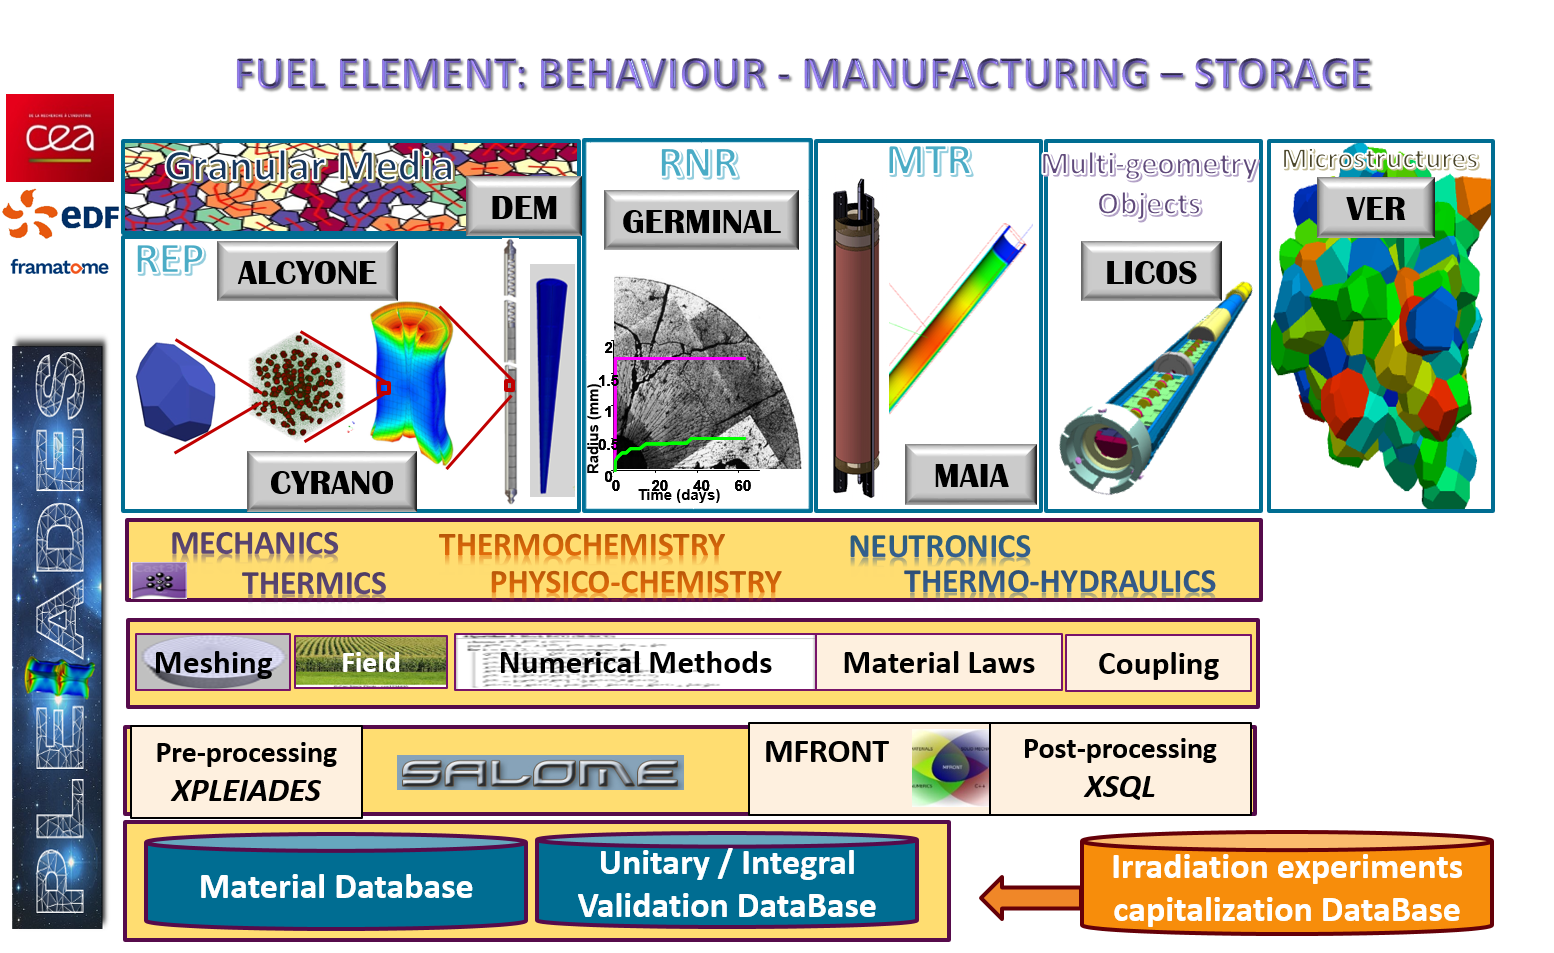
\includegraphics[trim = .2cm .2cm .2cm .6cm,clip,width=0.60\linewidth]{img/PLEIADES_2019_en.png}
    \vspace*{-3mm}
  \end{center}
  \begin{itemize}
    \item A wide range of materials (ceramics, metals, composites)
    \item A wide range of mechanical phenomena and behaviours
    \begin{itemize}
      \item Creep, swelling, irradiation effects, phase transitions ...
    \end{itemize}
    \item A wide range of mechanical loadings
  \end{itemize}
% Swelling, densification, relocation
% Creep, plasticity, fission gaz release
% Large strain, Contact
\begin{textblock}{.40}(0.11,0.24)
\scalebox{.7}{\rotatebox{90}{
    \begin{minipage}{7.cm}
      \center
  \textcolor{blue}{The Pleiades Platform}\\
  \textcolor{blue}{industrial partners: EDF, Framatome}
\end{minipage}}}
\end{textblock}

\begin{textblock}{.40}(0.84,0.22)
\scalebox{.7}{\rotatebox{90}{
\begin{minipage}{7.cm}
      \center
      \textcolor{red}{Existing mechanical solver}\\
      \textcolor{red}{not well parallelized}
\end{minipage}}}
\end{textblock}
\end{frame}

\Titre{Goals of \mmm{}\\[-1mm]
\hspace*{8mm}\scalebox{0.6}{\longmmm{}}}
\frame{
  \begin{itemize}
    \item Build a HPC general purpose non linear multi-physics
    library,\\
\hspace*{1cm}\textit{development began end of 2020.}
    \begin{itemize}
      \item Primary focus is \textbf{non linear solid mechanics} and
      \textbf{heat transfer}.
      \item Expected modelling (long-term): Shells, Beams,\\Phase-field
      approaches of brittle fracture, micromorphic models, Cosserat
      plasticity, strongly coupled thermo-chemical-mechanical or
      thermo-hydro-mechanical phenomena.
    \item Replace existing mechanical solver in Pleiades platform
    \item targeted application: microstructure and mesoscale modelling for nuclear fuel  
    \end{itemize}
\bigskip
    \item  A two-pillar library with \textit{opensource} commitment (\scalebox{0.8}{\mmm{} \textit{LGPL 3.0}}):
    \begin{itemize}
      \item \texttt{MFEM:} HPC finite element solver \scalebox{0.8}{\textit{(3-clause BSD)}}
      \item \texttt{MGIS/MFront:} constitutive laws, material modelling \scalebox{0.8}{\textit{(LGPL 3.0 / GPL 3.0)}}
    \end{itemize}
  \end{itemize}
}

\Titre{\scalebox{0.8}{Open-source orientation}\\\hspace*{8mm}\scalebox{0.8}{Expected benefits}}
\frame{
\scalebox{0.8}{
  \begin{minipage}{14.5cm}
    \begin{itemize}
    \item Exchanges and collaboration\\
    \begin{itemize}
    \item Facilitate sharing of reference solutions, standard benchmark problems and input data
    \item Foster collaboration with academics
    \item Allow to assess features and opportunities for integration of already developed open-source codes
    \item Ease the spread of the tool within industry, dodge the silos due to funding within companies
    \end{itemize}
\bigskip
    \item  Lesson learned from \texttt{MFront} developped at CEA\\\hspace*{1cm}opensource since 2014 (cf. poster session)
    \begin{itemize}
    \item ease the access to the tool: increase in visibility, reproducibility, credibility
    \item software engineering: users help to improve the software (bug report) and robustness
    \item other codes that use your product: opportunity for partnership, publications
    \item extra work, need to book time for: minimal user support, documentation, training
    \end{itemize}
  \end{itemize}
  \end{minipage}}
}

\section{A small tutorial}
\Intercalaire{A small tutorial}


\begin{frame}[fragile]{{\small What are we talking about ?}\\
\hspace*{1cm}{\small Example of end-user API}}
  \begin{center}
%    \scalebox{0.7}{
      \begin{minipage}{\linewidth}
      \tiny
      \begin{Highlighting}[]
        \CommentTok{// loading the mesh and building the non linear problem}
        \NormalTok{mfem_mgis::NonLinearEvolutionProblem problem(}
        \NormalTok{    \{\{}\StringTok{"MeshFileName"}\NormalTok{, mesh_file\},  \{}\StringTok{"FiniteElementFamily"}\NormalTok{, }\StringTok{"H1"}\NormalTok{\},}
        \NormalTok{     \{}\StringTok{"FiniteElementOrder"}\NormalTok{, order\}, \{}\StringTok{"UnknownsSize"}\NormalTok{, dim\},}
        \NormalTok{     \{}\StringTok{"Hypothesis"}\NormalTok{, }\StringTok{"PlaneStrain"}\NormalTok{\}, \{}\StringTok{"Parallel"}\NormalTok{, parallel\}\});}
        \CommentTok{// associating names to element and boundary attributes (could be automated for some mesh formats)}
        \NormalTok{problem.setMaterialsNames(\{\{1, }\StringTok{"NotchedBeam"}\NormalTok{\}\});}
        \NormalTok{problem.setBoundariesNames(\{\{3, }\StringTok{"LowerBoundary"}\NormalTok{\}, \{4, }\StringTok{"SymmetryAxis"}\NormalTok{\}, \{2, }\StringTok{"UpperBoundary"}\NormalTok{\}\});}
        \CommentTok{// declaring behaviour integrators}
        \NormalTok{problem.}\NormalTok{addBehaviourIntegrator}\NormalTok{(}\StringTok{"Mechanics"}\NormalTok{, }\StringTok{"NotchedBeam"}\NormalTok{, library, behaviour);}
        \CommentTok{// setting the initial state of the materials}
        \KeywordTok{auto}\NormalTok{\& m1 = problem.getMaterial(}\StringTok{"NotchedBeam"}\NormalTok{);}
        \NormalTok{mgis::behaviour::setExternalStateVariable(m1.s0, }\StringTok{"Temperature"}\NormalTok{, }\FloatTok{293.15}\NormalTok{);}
        \NormalTok{...}
        \CommentTok{// defining boundary conditions, postprocessings and solver parameters}
        \NormalTok{problem.addUniformDirichletBoundaryCondition(\{\{}\StringTok{"Boundary"}\NormalTok{, }\StringTok{"LowerBoundary"}\NormalTok{\}, \{}\StringTok{"Component"}\NormalTok{, 1\}\}\});}
        \NormalTok{problem.addPostProcessing(}\StringTok{"ParaviewExportResults"}\NormalTok{, \{\{}\StringTok{"OutputFileName"}\NormalTok{, }\StringTok{"ssna303-displacements"}\NormalTok{\}\})};
        \KeywordTok{auto}\NormalTok{\& solver = problem.getSolver();}
        \NormalTok{...}
        \CommentTok{// loop over time step}
        \ControlFlowTok{for}\NormalTok{ (mfem\_mgis::}\DataTypeTok{size\_type}\NormalTok{ i = }\DecValTok{0}\NormalTok{; i != nsteps; ++i) \{}
        \CommentTok{  // updating the boundary values and resolution}
        \NormalTok{  ...}
        \NormalTok{  problem.solve(dt);}
        \NormalTok{  problem.update();}
        \NormalTok{  t += dt;}
        \NormalTok{\}}
      \end{Highlighting}
    \end{minipage}
    %    }
  \end{center}
  \begin{itemize}
    \item Instantiating \scalebox{0.8}{\texttt{NonLinearEvolutionProblem}} class is the
    main entry point
    \item \textbf{Behaviour integrator} is the main new
    concept of {\tt MFEM/MGIS}
  \end{itemize}
\end{frame}

\section{Design and features of the \mmm{} project}
\Intercalaire{Design and features of the \mmm{} project}

\begin{frame}[fragile]{\texttt{MFEM} library}
\begin{itemize}
\item
  Main features \hspace*{2mm} {\small \url{https://mfem.org/}}
  \begin{itemize} 
  \item
    C++, opensource FEM library. Large community 
  \item
    \textbf{High-order} finite element meshes and spaces
  \end{itemize}
\end{itemize}
\vspace*{1mm}
\begin{itemize}
\item  \textbf{HPC} oriented
 \begin{itemize}
  \item
    Scales to hundreds of thousands of cores
  \item
    Many hardware devices are supported, such as GPUs
  \item
    Minimal changes to switch from serial to parallel version
  \item
    Top-notch optimizations for speeding up computations
  \item
    Able to call many standard linear solvers (Hypre, PETSC, \ldots)
  \end{itemize}
\end{itemize}
\vspace*{1mm}
\begin{itemize}
\item
  Mesh features
  \begin{itemize}
  \item
    Triangular, quadrilateral, tetrahedral, wedge, and hexahedral
    elements
  \item
    \textbf{Periodic} meshes
  \item
    Conforming and nonconforming adaptive mesh refinement
  \item
    Parallel \textbf{load balancing} (several methods)
  \end{itemize}
\end{itemize}
\vspace*{1mm}
\begin{itemize}
\item
  Non linear PDE's resolution
  \begin{itemize}
  \item
    handled by \textbf{non linear form integrators} which describes how
    to build the element contribution to the \emph{residual} and its
    \emph{jacobian}.\\
    \hspace*{0.333em}\hspace*{0.333em}Glue with \texttt{MGIS} is here
  \end{itemize}
\end{itemize}
\begin{textblock}{.15}(0.8,0.13)
    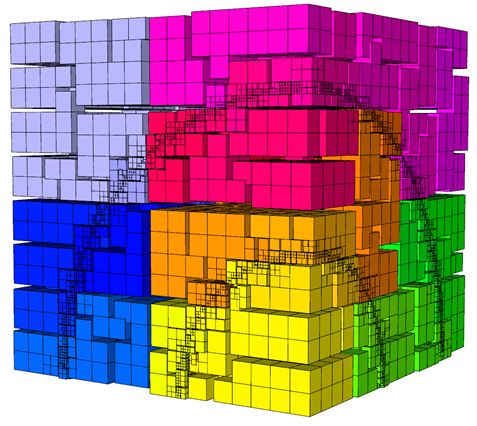
\includegraphics[width=\textwidth]{img/amr1.png}
\end{textblock}
\begin{textblock}{.19}(0.79,0.34)
    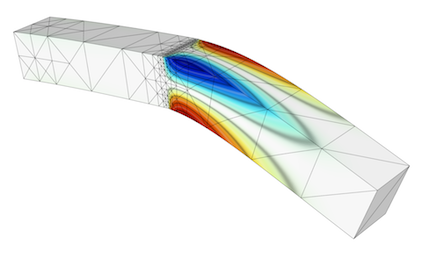
\includegraphics[width=\textwidth]{img/ex21.png}
\end{textblock}
\end{frame}

\begin{frame}[fragile]{Motivations for choosing \texttt{MFEM}}
\vspace*{2mm}
\scalebox{0.85}{
\begin{minipage}{1.15\linewidth}
\begin{itemize}
\item Many linear solvers available in \texttt{MFEM}
  \begin{itemize} 
  \item direct and iterative ones
  \item large set of preconditioners
  \item matrix-free approach
  \item GPU versions proposed
  \end{itemize}
\vspace*{.5mm}
\item Highly configurable through \texttt{spack} tool
 \begin{itemize}
  \item ease installation and configuration of the software stack
  \item helps to deal with complex settings and dependancies
  \item opensource and include recent versions of software
  \item bring performance and low maintenance efforts
  \end{itemize}
\vspace*{.5mm}
\item Software lifecycle
  \begin{itemize}
  \item the community helps to identify bugs and to propose solutions
  \item maintenance is offered
  \item access to release version (every year) and master version
  \end{itemize}
\vspace*{.5mm}
\item Opensource
  \begin{itemize}
  \item community of \texttt{MFEM} is large\\
  $\rightarrow$ brings extensive community support (github issues)
  \item license is compatible with our usage
  \item foster collaborations\\
  $\rightarrow$ MFEM workshop (cf s.13), EU project OperaHPC (cf s.14)
  \end{itemize}
\end{itemize}
\end{minipage}}

\begin{textblock}{.19}(0.8,0.72)
    
\includegraphics[trim = 0cm 1.5cm 0cm 1.cm,clip,width=\textwidth]{img/github.png}
\end{textblock}

\begin{textblock}{.24}(0.75,0.43)
    
\includegraphics[trim = 0cm 1.5cm 0cm 1.5cm,clip,width=\textwidth]{img/spack.jpg}
\end{textblock}

\end{frame}

\Titre{The \texttt{MFrontGenericInterfaceSupport} project}
\begin{frame}
  \begin{center}
    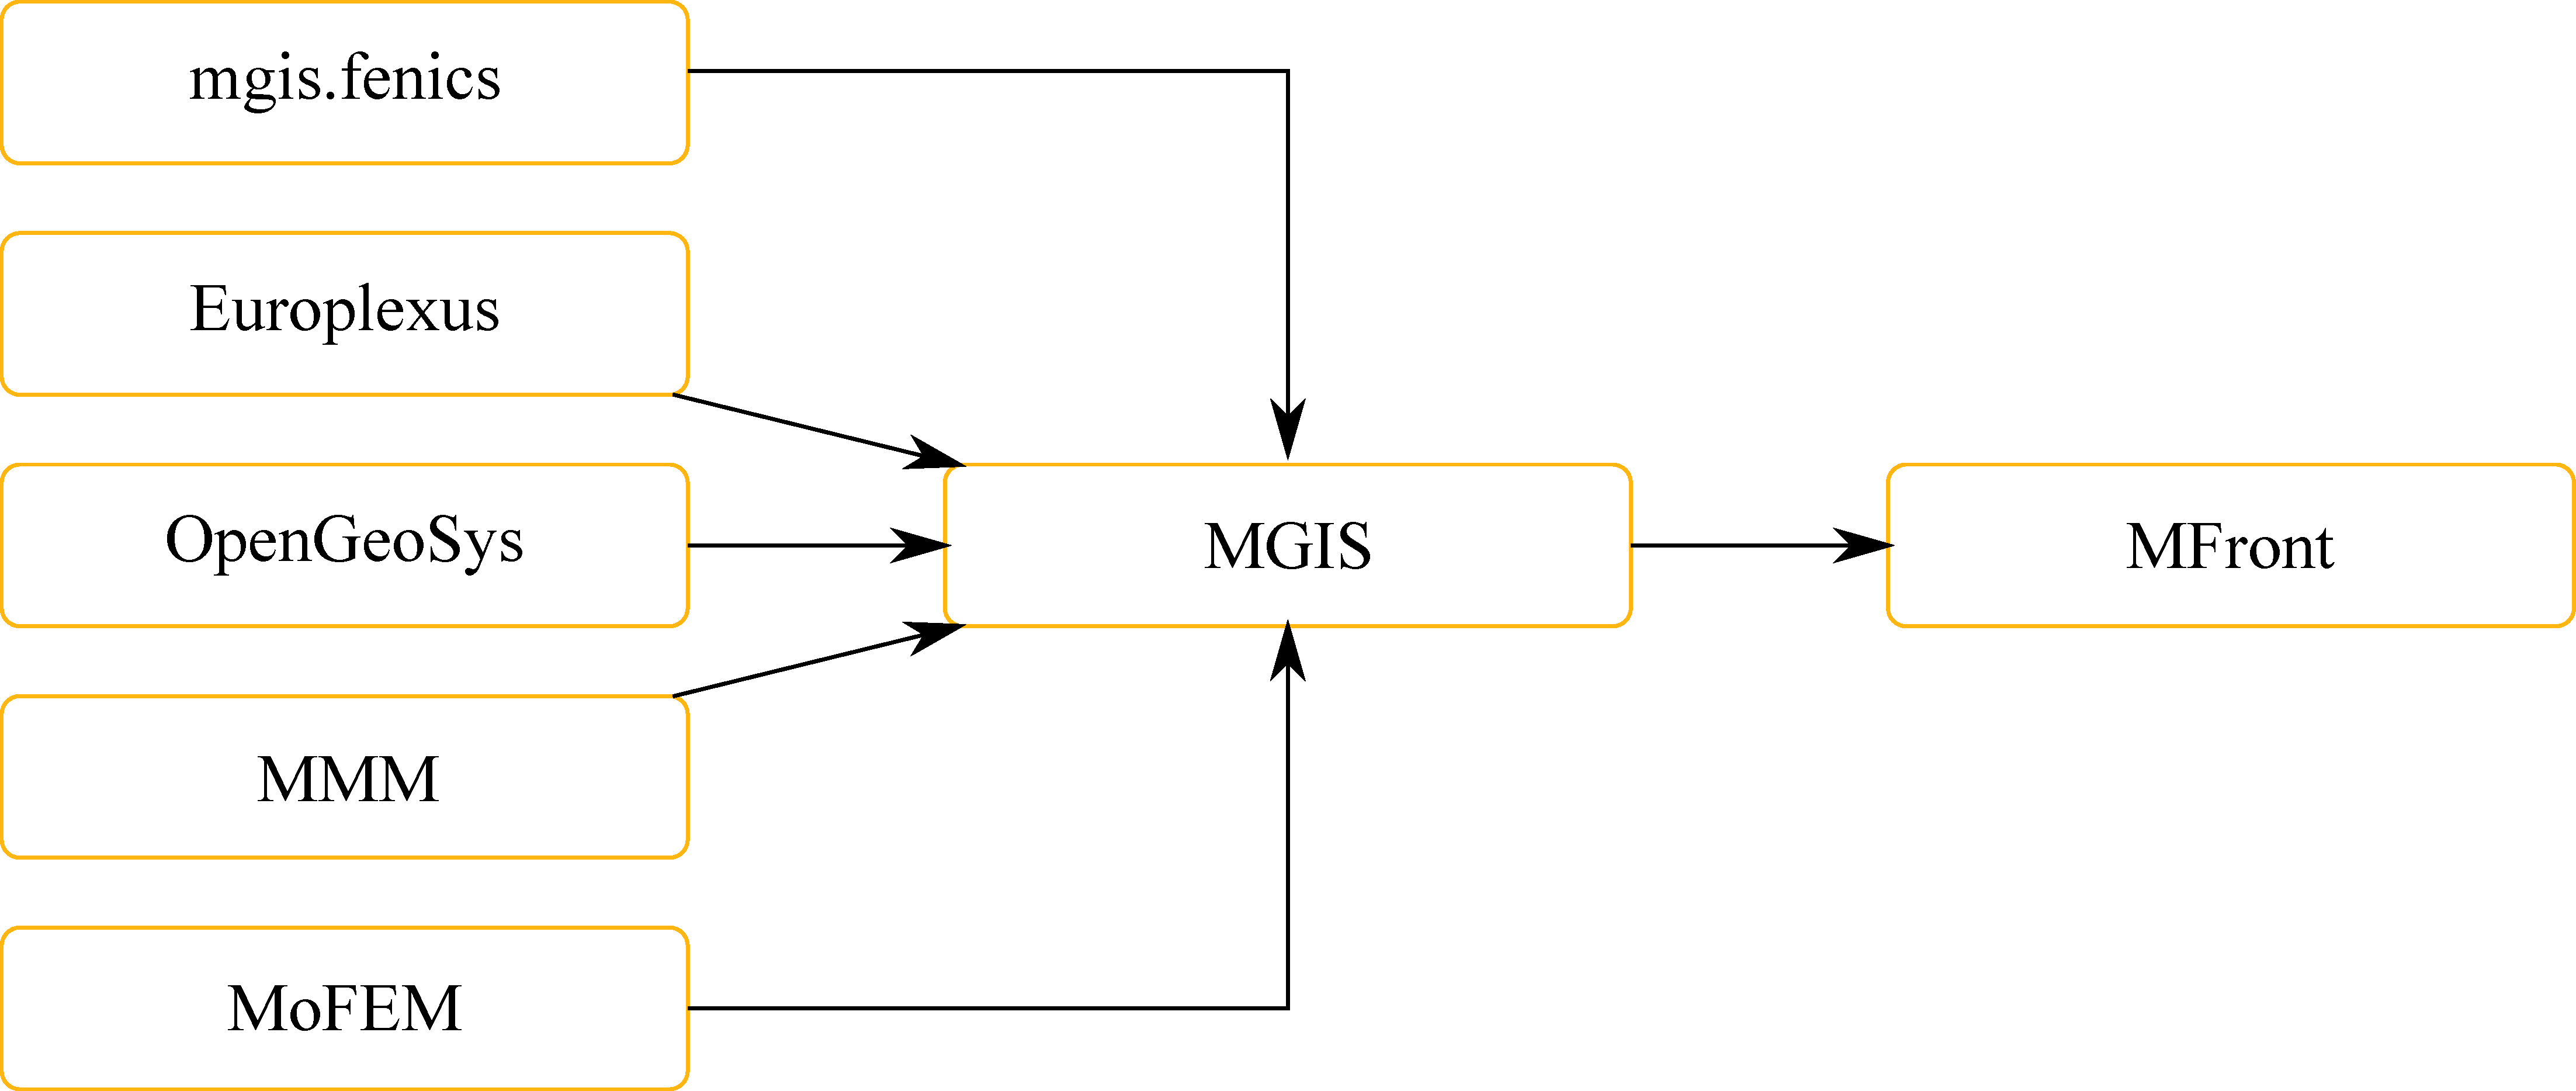
\includegraphics[width=0.75\textwidth]{img/mgis.pdf}
  \end{center}
  \scalebox{0.85}{
    \begin{minipage}{1.15\linewidth}
  \begin{itemize}
  \item High-level API to ease the use of MFront
  \begin{itemize}
  \item Provides classes to retrieve {\bf metadata} from an {\tt MFront} behaviour and
    call the behaviour integration over a time step
  \item Provides way to \textbf{ease memory management}: deal with internal state variables
  \item Written in \texttt{C++}, bindings exists for
    \texttt{C}, \texttt{Fortran2003}, \texttt{python}, \texttt{Julia}
  \end{itemize}
    \item Used/tested in \texttt{mgis.fenics},
    \texttt{OpenGeoSys}, \texttt{MMM}, \texttt{XPer}, \texttt{MoFEM},
    \texttt{Disk++}, \texttt{Kratos Multiphysics}, \texttt{JuliaFEM},
    \texttt{NairmMPM}, \texttt{esys.escript}, \texttt{DUNE},
    \texttt{OOFEM} ...
  \end{itemize}
  \end{minipage}}
\end{frame}

\begin{frame}[fragile]{The
    added value of \mmm{}\\\hspace*{8mm}\scalebox{0.6}{\longmmm{}}}
  \scalebox{0.85}{
    \begin{minipage}{1.2\linewidth}
  \begin{itemize}
    \item Statements
    \begin{itemize}
      \item \emph{Poor} support of multiple materials in
      \texttt{MFEM} for solid mechanics
      \item \emph{No} support for functions on integration
      points for a given material (element attribute)
    \end{itemize}
    \smallskip
    \item Improvements made by \mmm{}
    \begin{itemize}
      \item Support for non linear behaviour integrators
      based on \texttt{MFront}
      \item Support for functions on integration points that depends on
      material identifier
    \item Simplified High-level API for end users (mechanics)
    \item Support for the MED mesh file format (needed for EDF/CEA partnership)
    \item [TODO] Support for complex boundary conditions specific to nonlinear mechanics
    \end{itemize}
    \smallskip
    \item In practice, \mmm{} is a library made up of
      \begin{enumerate}
        
        \item Classes that inherit from \texttt{MFEM}\\\hspace*{6mm} loops
        on elements, linear \& non-linear solvers, mesh management\ldots{}
        \item Classes that inherit from \texttt{MGIS}\\\hspace*{6mm}
        materials management, internal variables, fill matrix
        entries\ldots{}
        \item Procedures for the end user to interact with MFEM
        \& MGIS
      \end{enumerate}
    \smallskip
    \item \mmm{} is a C++17 opensource library
    \begin{itemize}
      \item \url{https://github.com/thelfer/mfem-mgis}
      \item \url{https://github.com/latug0/mfem-mgis-examples}
    \end{itemize}
  \end{itemize}
  \end{minipage}}
\end{frame}

\begin{frame}{The
    role of behaviour integrators}
  \begin{center}
    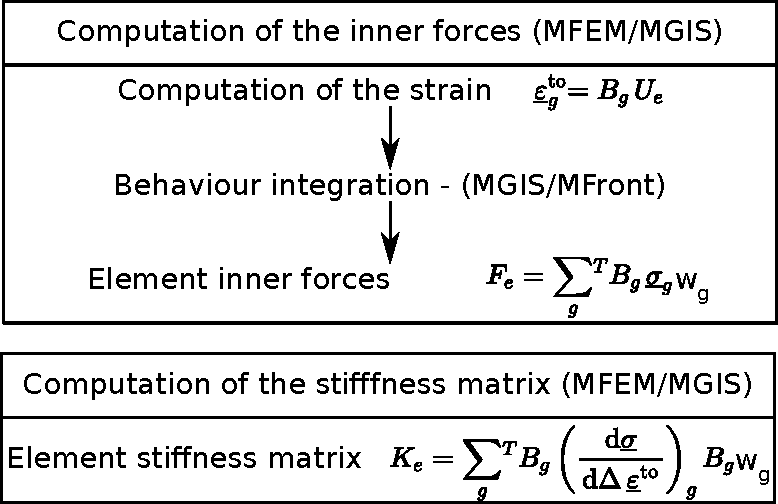
\includegraphics[width=0.6\textwidth]{img/behaviour-integrators.pdf}
  \end{center}
  \begin{itemize}
    \item Behaviour integrators are associated with a material
    identifier (element attribute).
    \item Behaviour integrators are called in the assembly loop
    over the elements for:
    \begin{itemize}
      \item the residual (contribution of the inner forces)
      \item the jacobian matrix (i.e.~the tangent stiffness
      matrix)
    \end{itemize}
  \end{itemize}
\end{frame}


%\begin{frame}[fragile]{Computation of the inner forces}
%  \protect\hypertarget{computation-of-the-inner-forces}{}
%  \begin{Shaded}
%    \begin{Highlighting}[]
%      \KeywordTok{template}\NormalTok{ \textless{}Hypothesis H\textgreater{}}
%      \DataTypeTok{void}\NormalTok{ SmallStrainMechanicalBehaviourIntegrator\textless{}H\textgreater{}::updateInnerForces(}
%      \NormalTok{      mfem::Vector \&Fe,}
%      \AttributeTok{const}\NormalTok{ mgis::span\textless{}}\AttributeTok{const}\NormalTok{ real\textgreater{} \&s,}
%      \AttributeTok{const}\NormalTok{ mfem::DenseMatrix \&dN,}
%      \AttributeTok{const}\NormalTok{ real w,}
%      \AttributeTok{const} \DataTypeTok{size\_type}\NormalTok{ ni) }\AttributeTok{const}\NormalTok{ \{}
%      \KeywordTok{constexpr} \AttributeTok{const} \KeywordTok{auto}\NormalTok{ icste = }\FloatTok{0.70710678118654752440}\NormalTok{;}
%      \KeywordTok{static\_assert}\NormalTok{(H == Hypothesis::TRIDIMENSIONAL, }\StringTok{"unsupported hypothesis"}\NormalTok{);}
%      \ControlFlowTok{if} \KeywordTok{constexpr}\NormalTok{ (H == Hypothesis::TRIDIMENSIONAL) \{}
%      \AttributeTok{const} \KeywordTok{auto}\NormalTok{ nnodes = dN.NumRows();}
%      \AttributeTok{const} \KeywordTok{auto}\NormalTok{ nx = ni;}
%      \AttributeTok{const} \KeywordTok{auto}\NormalTok{ ny = ni + nnodes;}
%      \AttributeTok{const} \KeywordTok{auto}\NormalTok{ nz = ni + }\DecValTok{2}\NormalTok{ * nnodes;}
%      \NormalTok{      real B[}\DecValTok{6}\NormalTok{][}\DecValTok{3}\NormalTok{] = \{\{dN(ni, }\DecValTok{0}\NormalTok{), }\DecValTok{0}\NormalTok{, }\DecValTok{0}\NormalTok{\},                          }\CommentTok{//}
%      \NormalTok{                      \{}\DecValTok{0}\NormalTok{, dN(ni, }\DecValTok{1}\NormalTok{), }\DecValTok{0}\NormalTok{\},                          }\CommentTok{//}
%      \NormalTok{                      \{}\DecValTok{0}\NormalTok{, }\DecValTok{0}\NormalTok{, dN(ni, }\DecValTok{2}\NormalTok{)\},                          }\CommentTok{//}
%      \NormalTok{                      \{dN(ni, }\DecValTok{1}\NormalTok{) * icste, dN(ni, }\DecValTok{0}\NormalTok{) * icste, }\DecValTok{0}\NormalTok{\},  }\CommentTok{// xy}
%      \NormalTok{                      \{dN(ni, }\DecValTok{2}\NormalTok{) * icste, }\DecValTok{0}\NormalTok{, dN(ni, }\DecValTok{0}\NormalTok{) * icste\},  }\CommentTok{// xz}
%      \NormalTok{                      \{}\DecValTok{0}\NormalTok{, dN(ni, }\DecValTok{2}\NormalTok{) * icste, dN(ni, }\DecValTok{1}\NormalTok{) * icste\}\}; }\CommentTok{// yz}
%      \NormalTok{      Fe[nx] += w * (B[}\DecValTok{0}\NormalTok{][}\DecValTok{0}\NormalTok{] * s[}\DecValTok{0}\NormalTok{] + B[}\DecValTok{1}\NormalTok{][}\DecValTok{0}\NormalTok{] * s[}\DecValTok{1}\NormalTok{] + B[}\DecValTok{2}\NormalTok{][}\DecValTok{0}\NormalTok{] * s[}\DecValTok{2}\NormalTok{] +}
%      \NormalTok{                     B[}\DecValTok{3}\NormalTok{][}\DecValTok{0}\NormalTok{] * s[}\DecValTok{3}\NormalTok{] + B[}\DecValTok{4}\NormalTok{][}\DecValTok{0}\NormalTok{] * s[}\DecValTok{4}\NormalTok{] + B[}\DecValTok{5}\NormalTok{][}\DecValTok{0}\NormalTok{] * s[}\DecValTok{5}\NormalTok{]);}
%      \NormalTok{      Fe[ny] += w * (B[}\DecValTok{0}\NormalTok{][}\DecValTok{1}\NormalTok{] * s[}\DecValTok{0}\NormalTok{] + B[}\DecValTok{1}\NormalTok{][}\DecValTok{1}\NormalTok{] * s[}\DecValTok{1}\NormalTok{] + B[}\DecValTok{2}\NormalTok{][}\DecValTok{1}\NormalTok{] * s[}\DecValTok{2}\NormalTok{] +}
%      \NormalTok{                     B[}\DecValTok{3}\NormalTok{][}\DecValTok{1}\NormalTok{] * s[}\DecValTok{3}\NormalTok{] + B[}\DecValTok{4}\NormalTok{][}\DecValTok{1}\NormalTok{] * s[}\DecValTok{4}\NormalTok{] + B[}\DecValTok{5}\NormalTok{][}\DecValTok{1}\NormalTok{] * s[}\DecValTok{5}\NormalTok{]);}
%      \NormalTok{      Fe[nz] += w * (B[}\DecValTok{0}\NormalTok{][}\DecValTok{2}\NormalTok{] * s[}\DecValTok{0}\NormalTok{] + B[}\DecValTok{1}\NormalTok{][}\DecValTok{2}\NormalTok{] * s[}\DecValTok{1}\NormalTok{] + B[}\DecValTok{2}\NormalTok{][}\DecValTok{2}\NormalTok{] * s[}\DecValTok{2}\NormalTok{] +}
%      \NormalTok{                     B[}\DecValTok{3}\NormalTok{][}\DecValTok{2}\NormalTok{] * s[}\DecValTok{3}\NormalTok{] + B[}\DecValTok{4}\NormalTok{][}\DecValTok{2}\NormalTok{] * s[}\DecValTok{4}\NormalTok{] + B[}\DecValTok{5}\NormalTok{][}\DecValTok{2}\NormalTok{] * s[}\DecValTok{5}\NormalTok{]);}
%      \NormalTok{    \}}
%      \NormalTok{  \}  }\CommentTok{// end of updateInnerForces}
%    \end{Highlighting}
%  \end{Shaded}
%  
%  \begin{itemize}
%    
%    \item
%    Note: code from the first versions of \texttt{mfem-mgis}
%    \item
%    The \texttt{B} matrix have numerous null entries.
%    
%    \begin{itemize}
%      
%      \item
%      The computation of \texttt{F} can easily be optimised.
%    \end{itemize}
%  \end{itemize}
%\end{frame}
%
%\begin{frame}[fragile]{Computation of the inner forces (optimized)}
%  \protect\hypertarget{computation-of-the-inner-forces-optimized}{}
%  \begin{Shaded}
%    \begin{Highlighting}[]
%      \KeywordTok{template}\NormalTok{ \textless{}Hypothesis H\textgreater{}}
%      \DataTypeTok{void}\NormalTok{ SmallStrainMechanicalBehaviourIntegrator\textless{}H\textgreater{}::updateInnerForces(}
%      \NormalTok{      mfem::Vector \&Fe,}
%      \AttributeTok{const}\NormalTok{ mgis::span\textless{}}\AttributeTok{const}\NormalTok{ real\textgreater{} \&s,}
%      \AttributeTok{const}\NormalTok{ mfem::DenseMatrix \&dN,}
%      \AttributeTok{const}\NormalTok{ real w,}
%      \AttributeTok{const} \DataTypeTok{size\_type}\NormalTok{ ni) }\AttributeTok{const}\NormalTok{ \{}
%      \KeywordTok{constexpr} \AttributeTok{const} \KeywordTok{auto}\NormalTok{ icste = }\FloatTok{0.70710678118654752440}\NormalTok{;}
%      \KeywordTok{static\_assert}\NormalTok{(H == Hypothesis::TRIDIMENSIONAL, }\StringTok{"unsupported hypothesis"}\NormalTok{);}
%      \ControlFlowTok{if} \KeywordTok{constexpr}\NormalTok{ (H == Hypothesis::TRIDIMENSIONAL) \{}
%      \AttributeTok{const} \KeywordTok{auto}\NormalTok{ nnodes = dN.NumRows();}
%      \AttributeTok{const} \KeywordTok{auto}\NormalTok{ nx = ni;}
%      \AttributeTok{const} \KeywordTok{auto}\NormalTok{ ny = ni + nnodes;}
%      \AttributeTok{const} \KeywordTok{auto}\NormalTok{ nz = ni + }\DecValTok{2}\NormalTok{ * nnodes;}
%      \NormalTok{      real B[}\DecValTok{6}\NormalTok{][}\DecValTok{3}\NormalTok{] = \{\{dN(ni, }\DecValTok{0}\NormalTok{), }\DecValTok{0}\NormalTok{, }\DecValTok{0}\NormalTok{\},                          }\CommentTok{//}
%      \NormalTok{                      \{}\DecValTok{0}\NormalTok{, dN(ni, }\DecValTok{1}\NormalTok{), }\DecValTok{0}\NormalTok{\},                          }\CommentTok{//}
%      \NormalTok{                      \{}\DecValTok{0}\NormalTok{, }\DecValTok{0}\NormalTok{, dN(ni, }\DecValTok{2}\NormalTok{)\},                          }\CommentTok{//}
%      \NormalTok{                      \{dN(ni, }\DecValTok{1}\NormalTok{) * icste, dN(ni, }\DecValTok{0}\NormalTok{) * icste, }\DecValTok{0}\NormalTok{\},  }\CommentTok{// xy}
%      \NormalTok{                      \{dN(ni, }\DecValTok{2}\NormalTok{) * icste, }\DecValTok{0}\NormalTok{, dN(ni, }\DecValTok{0}\NormalTok{) * icste\},  }\CommentTok{// xz}
%      \NormalTok{                      \{}\DecValTok{0}\NormalTok{, dN(ni, }\DecValTok{2}\NormalTok{) * icste, dN(ni, }\DecValTok{1}\NormalTok{) * icste\}\}; }\CommentTok{// yz}
%      \NormalTok{      Fe[nx] += w * (B[}\DecValTok{0}\NormalTok{][}\DecValTok{0}\NormalTok{] * s[}\DecValTok{0}\NormalTok{] + B[}\DecValTok{3}\NormalTok{][}\DecValTok{0}\NormalTok{] * s[}\DecValTok{3}\NormalTok{] + B[}\DecValTok{4}\NormalTok{][}\DecValTok{0}\NormalTok{] * s[}\DecValTok{4}\NormalTok{]);}
%      \NormalTok{      Fe[ny] += w * (B[}\DecValTok{1}\NormalTok{][}\DecValTok{1}\NormalTok{] * s[}\DecValTok{1}\NormalTok{] + B[}\DecValTok{3}\NormalTok{][}\DecValTok{1}\NormalTok{] * s[}\DecValTok{3}\NormalTok{] + B[}\DecValTok{5}\NormalTok{][}\DecValTok{1}\NormalTok{] * s[}\DecValTok{5}\NormalTok{]);}
%      \NormalTok{      Fe[nz] += w * (B[}\DecValTok{2}\NormalTok{][}\DecValTok{2}\NormalTok{] * s[}\DecValTok{2}\NormalTok{] + B[}\DecValTok{4}\NormalTok{][}\DecValTok{2}\NormalTok{] * s[}\DecValTok{4}\NormalTok{] + B[}\DecValTok{5}\NormalTok{][}\DecValTok{2}\NormalTok{] * s[}\DecValTok{5}\NormalTok{]);}
%      \NormalTok{    \}}
%      \NormalTok{  \}  }\CommentTok{// end of updateInnerForces}
%    \end{Highlighting}
%  \end{Shaded}
%  
%  \begin{itemize}
%    
%    \item
%    Note: code from the first versions of \texttt{mfem-mgis}
%  \end{itemize}
%\end{frame}

\begin{frame}{Behaviour
    integrators}
  \begin{itemize}
    \item Behaviour integrators are meant to
    \begin{itemize}
      \item Compute the gradients from unknowns (using the
      \(B\) matrix)
      \item Handle the state variables
      \item Call the behaviour integration
      \item Compute the inner forces from the thermodynamic
      forces
      \item Compute the stiffness matrix from the consistent
      tangent operator
    \end{itemize}
  \end{itemize}
  \begin{itemize}
    \item All those steps depends on
    \begin{itemize}
      \item Kind of problem described (mechanics, heat
      transfer)
      \item Symmetry of the material (isotropic or
      orthotropic)
      \item Modelling hypotheses: \(3D\), plane strain,
      plane stress, axisymmetry \ldots
    \end{itemize}
  \end{itemize}
  \begin{itemize}
    \item The writting of behaviour integrators is tedious and
    error-prone and shall be done with care
    \begin{itemize}
      \item However, specific behaviour integrators gives
      access to pieces of physics
      \item Code generation to the rescue !
    \end{itemize}
  \end{itemize}
\end{frame}

\begin{frame}[fragile]{The
    \texttt{behaviour-integrator} code
    generator}
  \begin{itemize}
    \item Aim of this code-generator
    \begin{itemize}
      \item Generate behaviour integrators from definition of the gradients
      \item Automated code factorisation/optimisation (no sparse matrix multiply)
      \item Avoid coding errors due to tedious formula
    \end{itemize}
    \item Machinery
    \begin{itemize}
      \item Based on the \texttt{GiNaC} for symbolic
      computations in \texttt{C++}
      \item Current scope: isotropic and orthotropic, small
      and finite strain behaviours in plane strain, plane stress and
      tridimensional hypotheses
    \end{itemize}
    \item Extensions (to come)
    \begin{itemize}
      \item Support of axisymmetry
      \item Non linear heat transfer, non linear diffusion
      \item Can be extended to other non-linear models, wide
      range of phenomena
    \end{itemize}
  \end{itemize}
\end{frame}

\section{Feed-backs on some issues using {\tt MFEM}}
\Intercalaire{Feed-backs on some issues using {\tt MFEM}}

\Titre{Issues related to {\tt MFEM}}
\frame{
  \scalebox{0.82}{
  \begin{minipage}{1.2\linewidth}
  \begin{itemize}
  \item Non-linear solve, integration step
  \begin{itemize}
    \item The integration of the mechanical behaviour is a {\bf
      complex} kernel solving a system of ordinary differential
    equations which can {\bf fail} -> not handled in MFEM
    \item Work-around: derived our own Newton
    algorithm which separates the behaviour integration step from
    residual/stiffness assemblies (however, does {\bf not work} with {\tt
        PETSc})
    \item Discussion started:
    \begin{itemize}
      \item \url{https://github.com/mfem/mfem/issues/2139}
      \item Also discussed during MFEM user meeting (20/10/2021) 
    \end{itemize}
  \end{itemize}
  \item Dirichlet boundary conditions
  \begin{itemize}
    \item Imposing the boundary Dirichlet in {\tt MFEM} leads
      to \textbf{unphysically strain} increments on elements near the boundary
      (exacerbated for refined mesh) -> divergence.
    \item In most \textbf{mechanical} solvers, a \textbf{prediction} of the
    solution based on the tangent problem is performed, not easy to do in MFEM
    \item Discussion started:
    \begin{itemize}
      \item \url{https://github.com/mfem/mfem/issues/2174}
      \item Also discussed during MFEM user meeting (20/10/2021)
    \end{itemize}
  \end{itemize}
\end{itemize}
\end{minipage}}
\begin{center}
  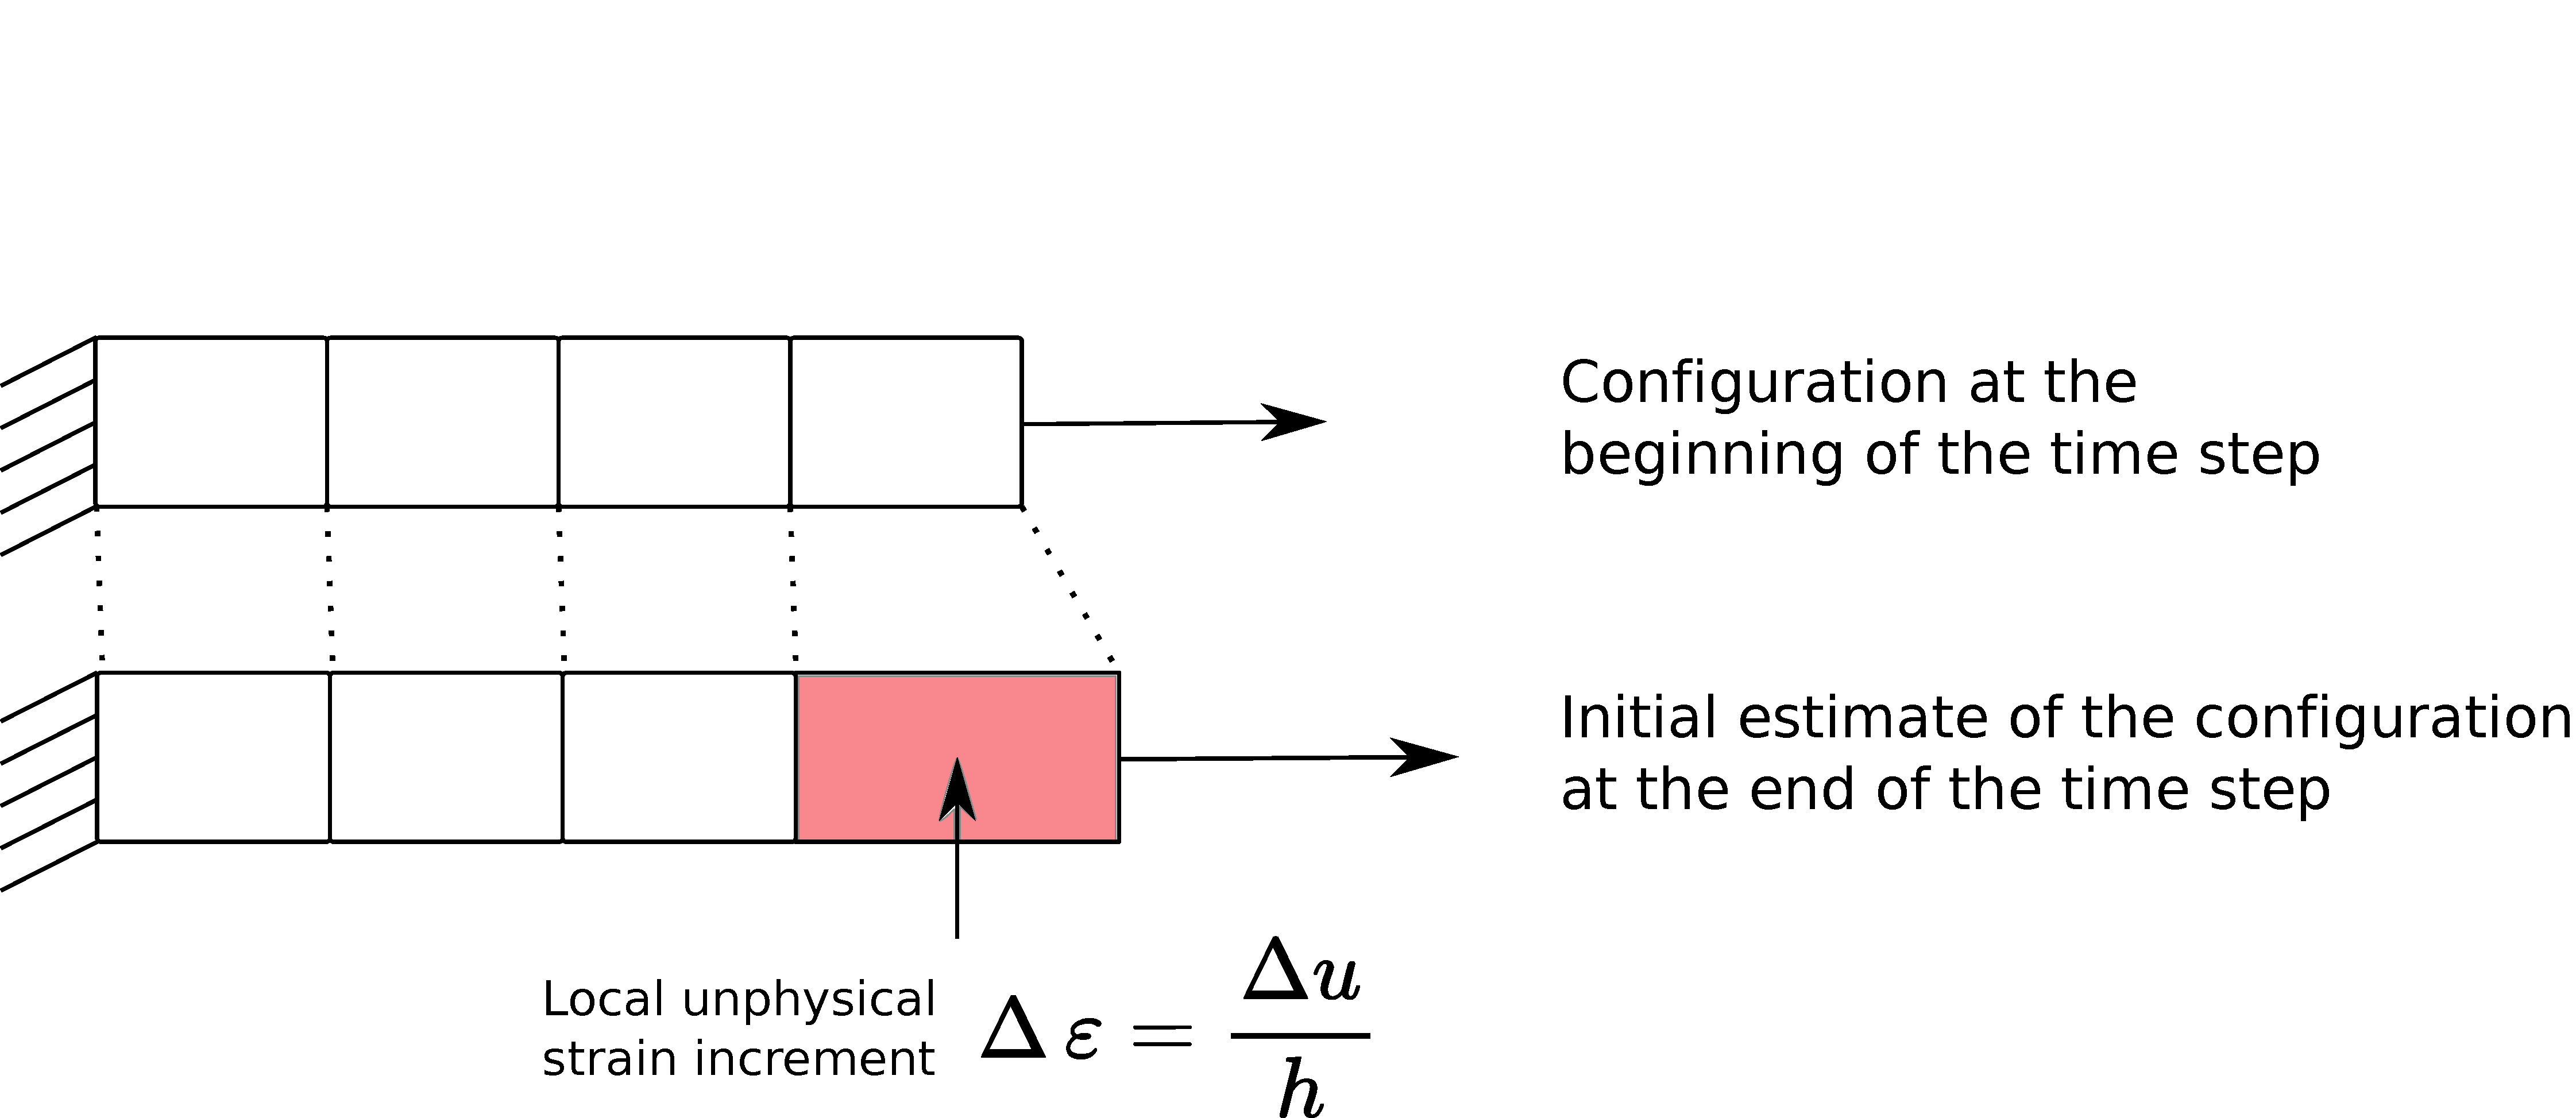
\includegraphics[trim = 0cm .1cm 0cm 0cm,clip,width=0.56\textwidth]{img/DirichletBoundaryConditionIssue.pdf}
\end{center}
}


\section{European project - OperaHPC}
\Intercalaire{European project - OperaHPC}

\begin{frame}{{\small OperaHPC}\\\hspace*{1cm}{\footnotesize OPEn HPC theRmo-mechanical tools for the development of eAtf fuels}}
\begin{textblock}{.94}(0.02,0.1)
  \begin{block}{European project}
    \small
    \begin{itemize}
      \itemsep 0pt
      \parskip 0pt
      \item Duration nov 2022 -> 2027
      \item Focus: Advanced simulation tools enabling \textbf{3D representation} of fuel rod
      \item Consortium: France, Italy, UK, Switzerland, Czech Republic, Sweden ...
    \end{itemize}
  \end{block}
\end{textblock}
\begin{textblock}{.94}(0.02,0.34)
  \begin{block}{Aims}
    \small
    \begin{itemize}
      \itemsep 0pt
      \parskip 0pt
    \item \textbf{Open-source} tools enabling direct or indirect use in \textbf{industrial} context
    \item Research \& training activities, better \textbf{knowledge} of fuel rods \& fuel behavior
    \item Support for \textbf{safe operation} of existing nuclear power plants
    \item \textbf{Physically-based} modelling implemented in HPC 3D simulation tools
    \end{itemize}
  \end{block}
\end{textblock}
\begin{textblock}{.7}(0.36,0.64)
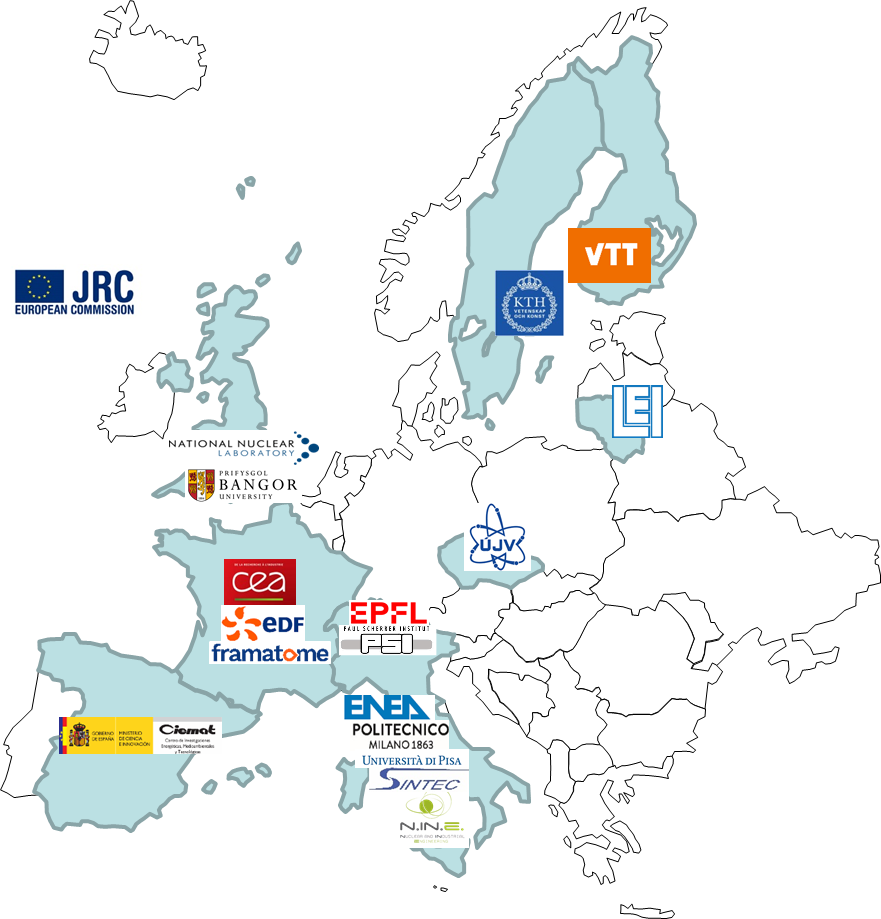
\includegraphics[trim = .1cm .25cm .02cm 1.1cm,clip,width=3cm]{img/members_operahpc.png}
%\hspace*{7mm}\scalebox{0.8}{\footnotesize Consortium}
\end{textblock}
\end{frame}


\begin{frame}{{\small OperaHPC}\\\hspace*{1cm}{\small Big picture}}
\begin{textblock}{.94}(0.02,0.1)
  \scalebox{0.85}{
    \begin{minipage}{1.16\linewidth}
  \begin{block}{Open-source benefits}
    \small
    \begin{itemize}
      \itemsep 0pt
      \parskip 0pt
    \item Open science approach: education/training, ease publication \& \textbf{dissemination}\\
      \hspace*{6mm} avoiding \textit{black-box} approaches
      
      \item Use \textbf{top-notch} opensource software \textbf{stacks}
      \item Ease the \textbf{coupling} of multiple codes within the consortium
      \item Helps promoting advanced HPC tools within nuclear community
      \item \textbf{Societal impact}: enable european citizen to know about tools used in nuclear field
    \end{itemize}
  \end{block}
  \end{minipage}}
\end{textblock}
\begin{textblock}{.4}(0.2,0.4)
 \center
\begin{overlayarea}{\textwidth}{\textheight}
\begin{tikzpicture}
\node[anchor=south west,inner sep=0] (image) at (0,0) {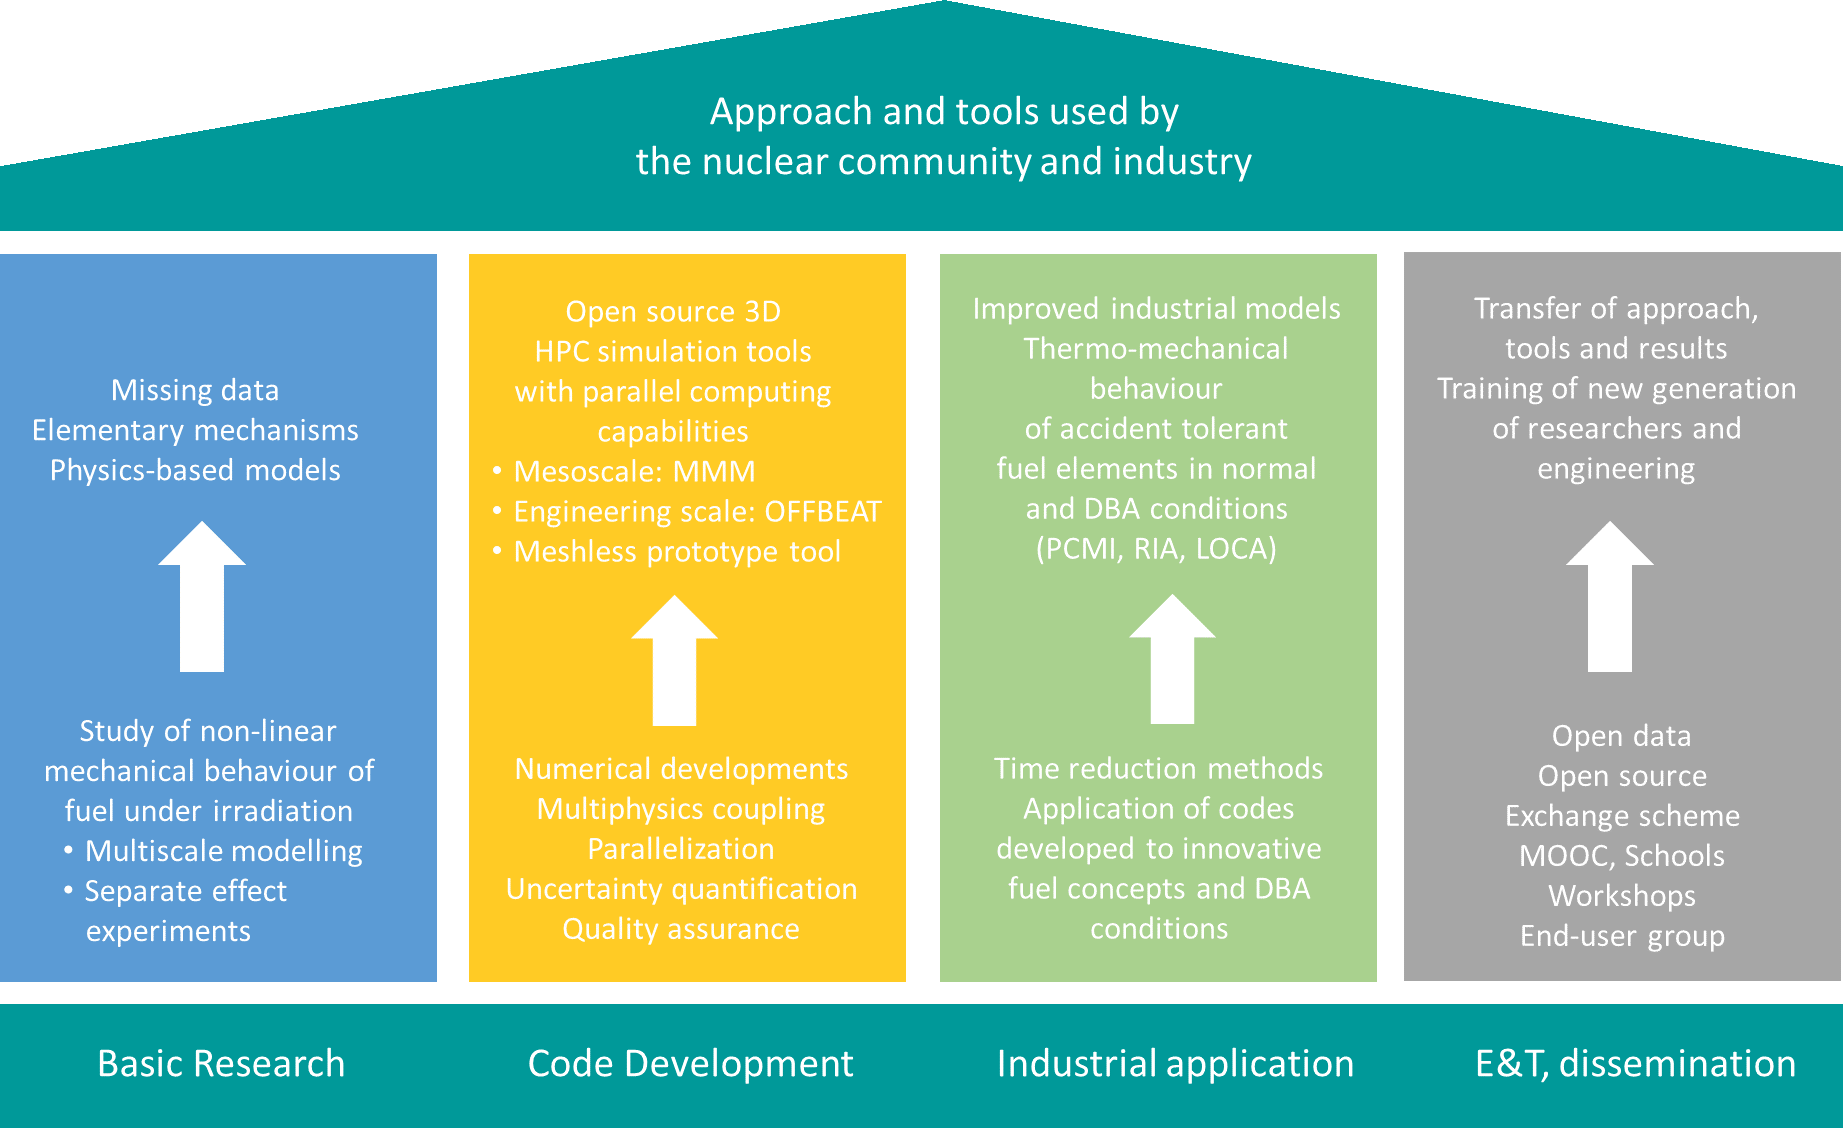
\includegraphics[keepaspectratio = true,width=7.5cm]{img/overall_operahpc_scheme.png}};
\draw [thick, red] (2.9,2.7) ellipse (.3 and 0.16) ;  
% coordinates, I do not have your original picture
\end{tikzpicture}
\end{overlayarea}

\scalebox{0.8}{\footnotesize Schematics of OperaHPC}
\end{textblock}
\end{frame}

\section{Examples}
\Intercalaire{Examples}

\begin{frame}{Non linear case \\\hspace*{1cm} Elastoplastic modelling, finite strain}
\begin{textblock}{.9}(0.02,0.1)
  \begin{block}{Case description}
    \begin{itemize}
      \item Uniaxial tensile test on a 3D notched beam
      \item Imposed displacement: right of the beam
      \item Symmetry conditions at: left position, down position 
    \end{itemize}
  \end{block}
\end{textblock}
\begin{textblock}{.4}(0.,0.5)
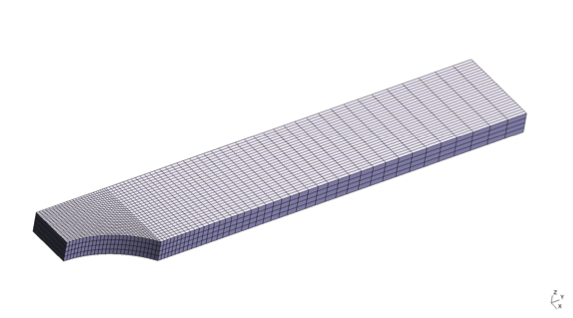
\includegraphics[width=0.9\textwidth]{img/ssna303-geom.png}\\
\hspace*{3mm}{\footnotesize Geometry of the notched beam}
\end{textblock}
\begin{textblock}{.61}(0.39,0.37)
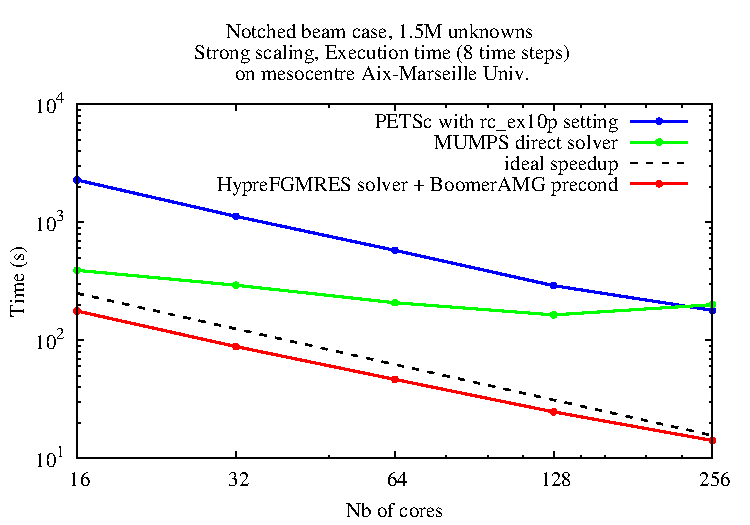
\includegraphics[trim = .1cm .1cm .1cm .1cm,clip,width=\textwidth]{bench/scal_ssna303.pdf}
\end{textblock}
\end{frame}


\begin{frame}{\scalebox{0.8}{Periodic
    Representative Elementary Volume  (REV)}\\\hspace*{1cm}
    \scalebox{0.8}{Pratical setting}}
  \scalebox{0.8}{
    \begin{minipage}{1.2\linewidth}
  \begin{block}{REV modelling in PLEIADES}
    \begin{itemize}
    \item Existing capabilities - not in \mmm{} but using previous Cast3m solver
    \begin{itemize}
      \item Microstructural representation:\\\hspace*{7mm} inclusions, polycrystals, coated materials
      \item Application:\\\hspace*{7mm} MOX fuel, Accident-Tolerent-Fuel (ATF), Thermal conductivity at fine scale
      \item Features: Damage, creep, homogenisation, cracking, multi-material, porosity $\ldots$
      \item Typical scale of computational domain: 500 $\mu{}m$
      \item Requirements: Periodic 3D boundary conditions
    \end{itemize}
      \item Aim: port these capabilities into \mmm{}
    \end{itemize}
  \end{block}
  \end{minipage}}

\vspace*{2mm}
\hspace*{1cm}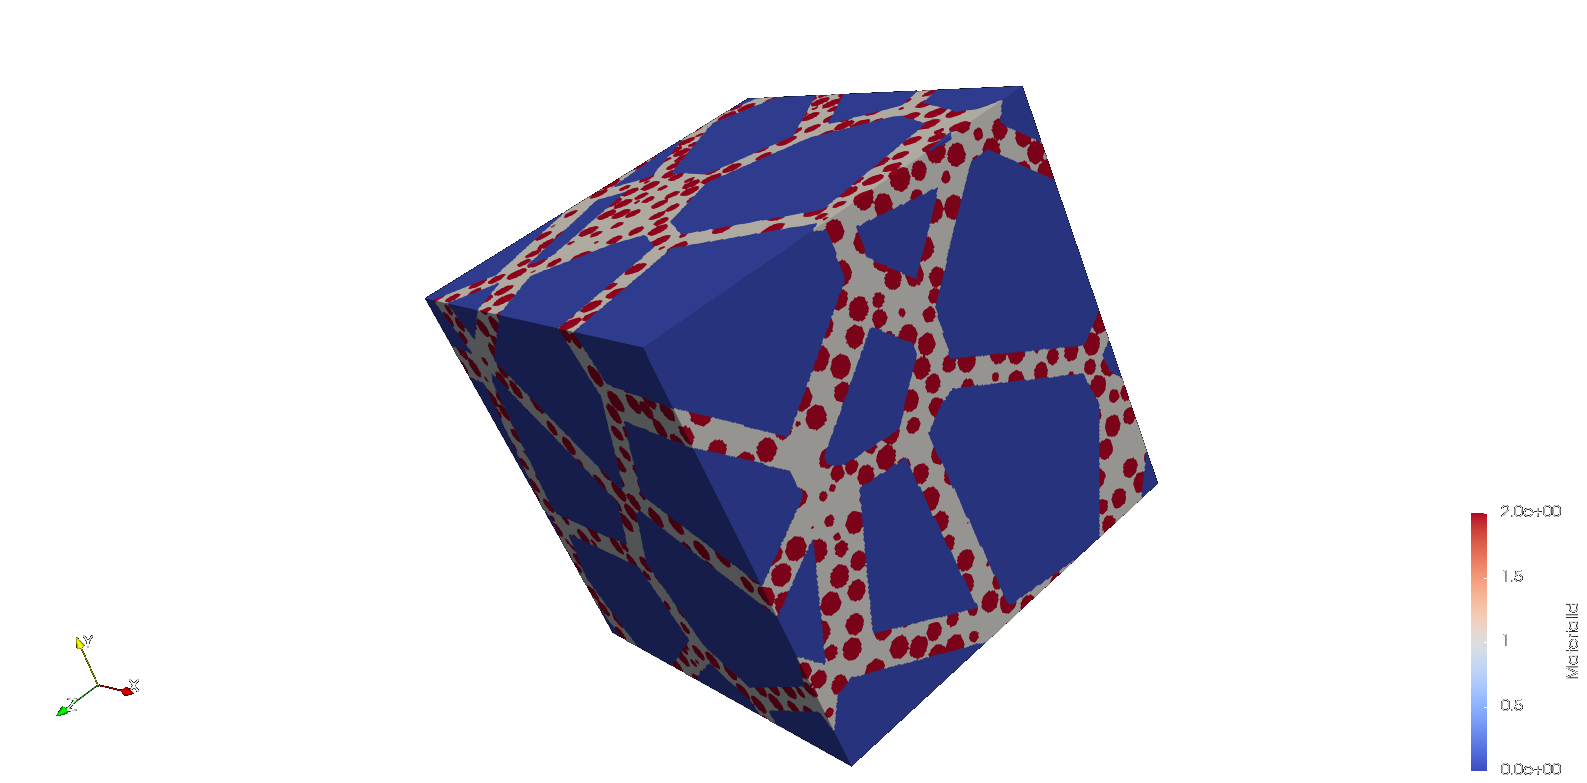
\includegraphics[width=2.5cm]{ver/Laguerre_Filamentaire1.png}
\hspace*{2mm}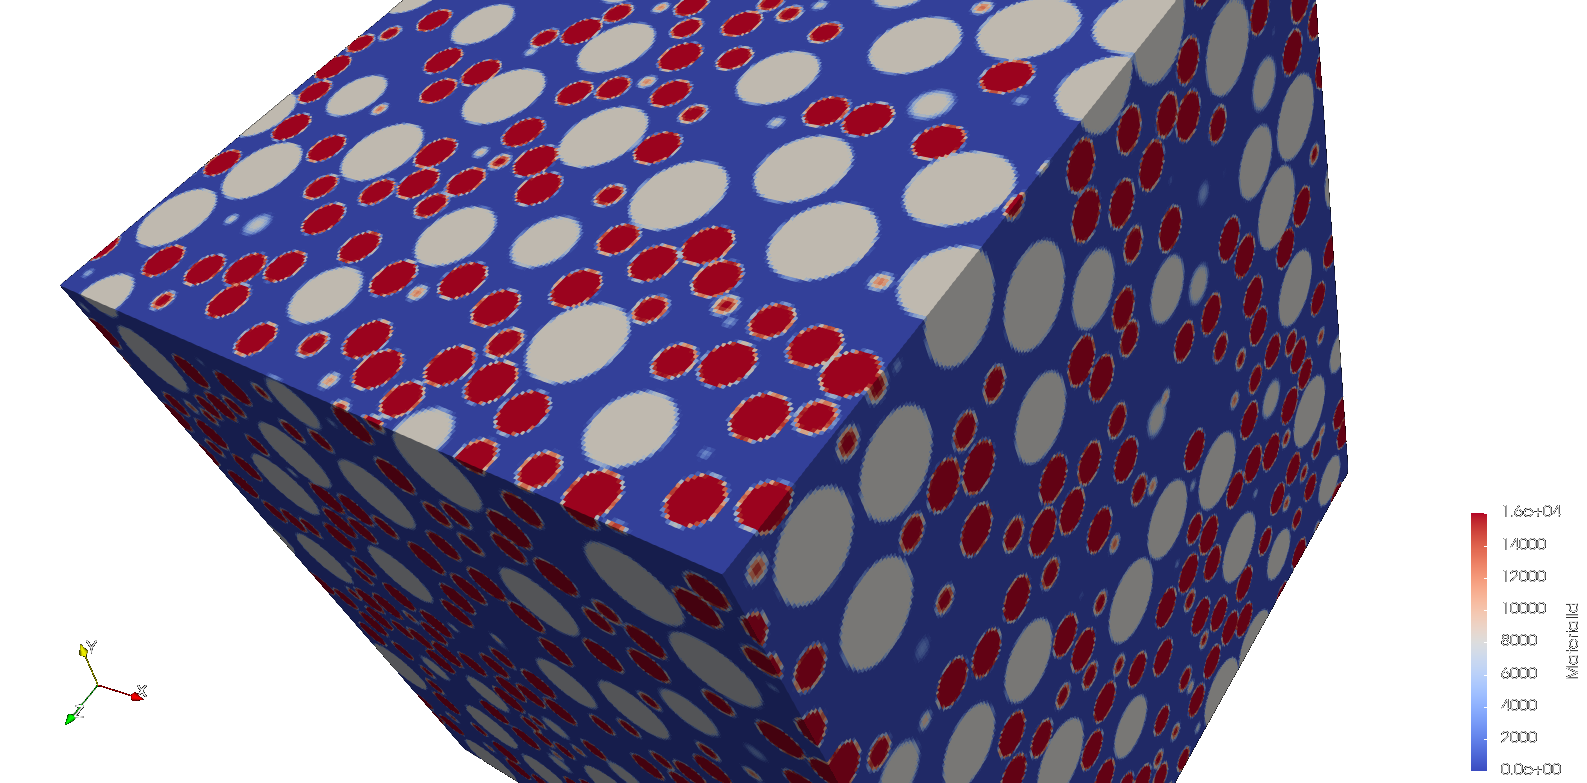
\includegraphics[width=2.5cm]{ver/Voxels_composites1.png}
%\includegraphics[width=0.38cm]{ver/Poly_2D.png}
\hspace*{2mm}\includegraphics[width=2.5cm]{ver/Mask_final1.png}
\\
\hspace*{1cm}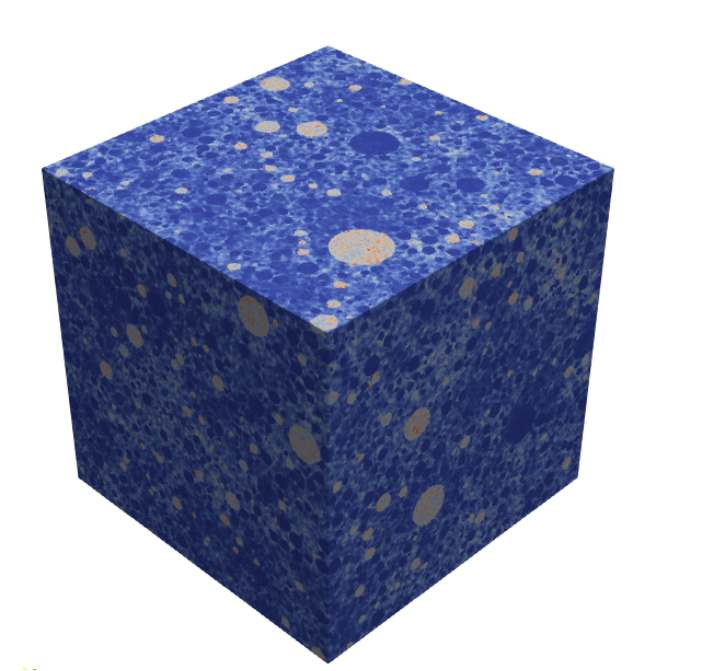
\includegraphics[width=2.5cm]{ver/Chps_Gauss.png}
\hspace*{2mm}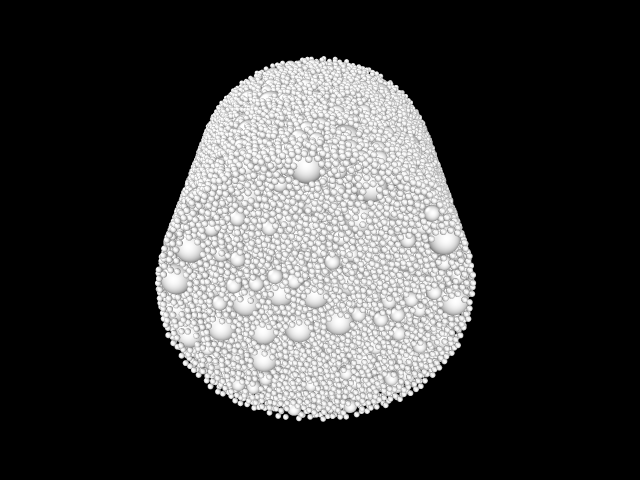
\includegraphics[width=2.5cm]{ver/Cylinder_3D.png}
\hspace*{2mm}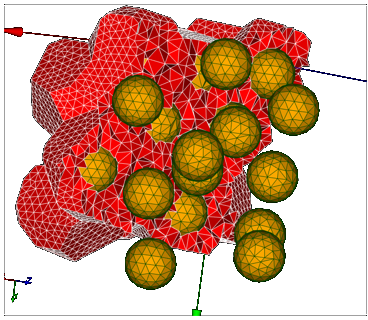
\includegraphics[trim = .1cm .1cm .1cm .1cm,clip,width=2.5cm]{ver/Maillage_vraiment_periodique1.png}
\end{frame}

\begin{frame}{\scalebox{0.8}{Periodic REV}\\\hspace*{1cm}\scalebox{0.8}{Numerical results on 32 cores for \mmm{}}}
  \begin{block}{Properties}
    \begin{itemize}
      \item 14 million unknowns, elastic modelling
      \item Ref. case on \emph{32 cores} - skylake @
      mesocentre Aix-Marseille University
      \item Main linear solver: Conj. Gradient (iterative),
      no preconditioner used
    \end{itemize}
  \end{block}
  \vspace*{2mm}
  \begin{block}{Timings}
    \begin{itemize}
      \item MFEM linear solve
      \begin{itemize}
        \item total \textbf{166s}, ~~ matrix assembly 39s,
        ~~ CGsolver 120s
      \end{itemize}
      \item MFEM non-linear solve - residual form, a single
      newton iteration
      \begin{itemize}
        \item total \textbf{179s}, ~~ matrix assembly 53s,
        ~~ CGsolver 117s
      \end{itemize}
      \item \mmm{} non-linear solve - residual form, a
      single newton iteration
      \begin{itemize}
        \item total \textbf{188s}, ~~ matrix assembly 42s,
        ~~ CGsolver 133s
      \end{itemize}
      \item Overheads due to \mmm{} are low
      \begin{itemize}
        \item Due to: read/write to memory buffers,
        function calls for assembly
      \end{itemize}
    \end{itemize}
  \end{block}
\end{frame}

\begin{frame}{\scalebox{0.8}{Periodic REV}\\\hspace*{1cm}\scalebox{0.8}{Strong Scaling}}
  \begin{block}{Strong
      scaling}
    \begin{itemize}
      \item Using \mmm{} non-linear solve
      \item Strong scaling from 32 to 256 cores
      \item Scalable parallelism observed (mainly due to MFEM capabilities)
    \end{itemize}
  \end{block}
  \begin{block}{}
    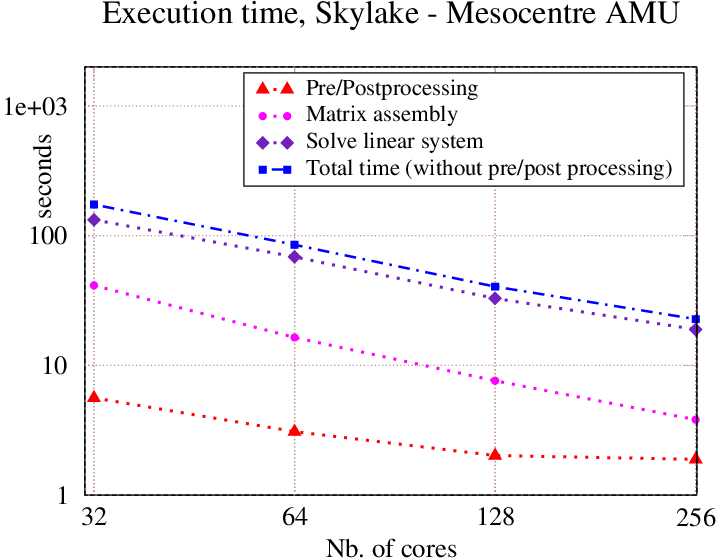
\includegraphics[width=0.4\textwidth]{img/bench_3.png}
    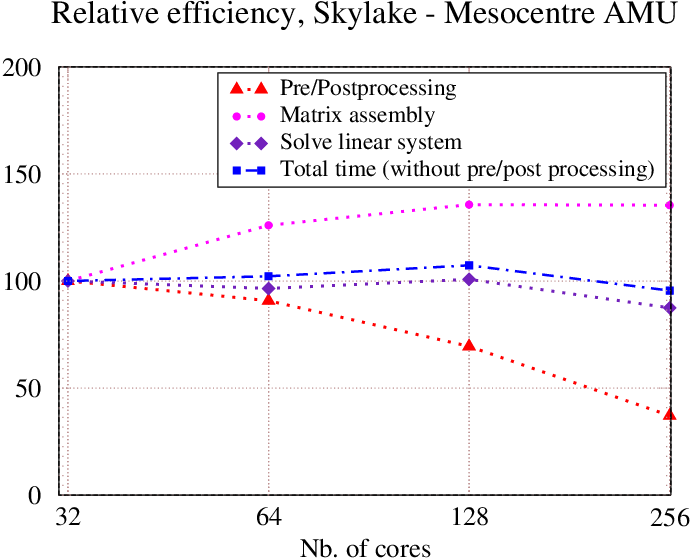
\includegraphics[width=0.4\textwidth]{img/bench_4.png}
  \end{block}
\end{frame}

\begin{frame}{\scalebox{0.8}{Periodic REV}\\\hspace*{1cm}\scalebox{0.8}{Modelling inclusions}}
  \begin{block}{Modelling inclusions at fuel pellet's microstructure scale}
    \hspace*{2cm}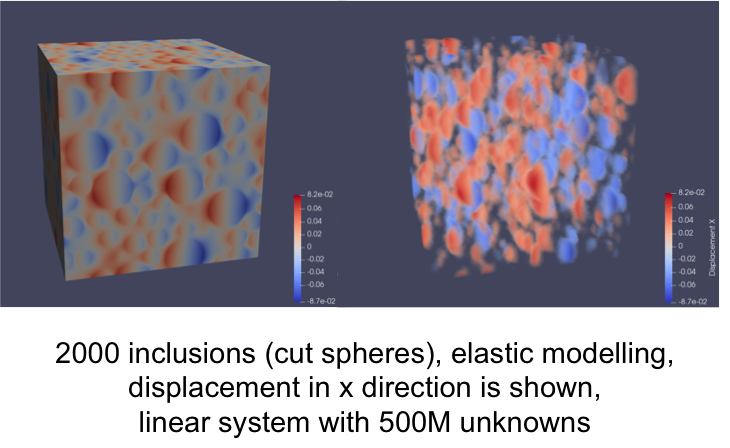
\includegraphics[height=4cm]{img/REV_2000inc.png}
  \end{block}
  \scalebox{0.9}{
    \begin{minipage}{1.1\linewidth}
  \begin{block}{MFEM contributions}
    \begin{itemize}
      \item Using as input : 3D periodic \texttt{gmsh} meshes\\[-1mm]
      \hspace*{8mm}\scalebox{0.8}{we made a public MFEM contribution to add these capabilities} 
      \item Read/write MED (Salome platform) I/O file format\\[-1mm]
      \hspace*{8mm}\scalebox{0.8}{development is not publicly disclosed}\\[-1mm]
      \hspace*{8mm}\scalebox{0.8}{pull request is delayed, need time to go through}
%      \item In progress : using \texttt{gmsh} to generate large REV meshes (\texttt{gmsh} format)\\[-1mm]
%      \hspace*{8mm}\scalebox{0.8}{including second order meshes} 
    \end{itemize}
  \end{block}
  \end{minipage}}
\begin{textblock}{.2}(0.73,0.22)
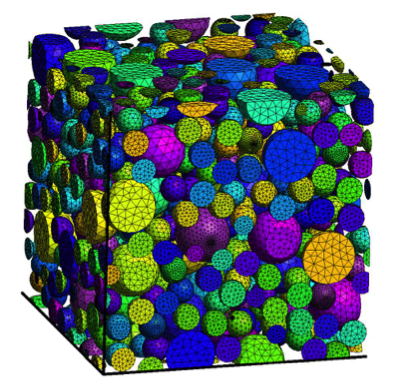
\includegraphics[width=\textwidth]{img/polydisperse.png}
\end{textblock}
\end{frame}

\begin{frame}{Periodic
    REV\\\hspace*{1cm}{\small Large runs on 65k cores}}
\begin{textblock}{.92}(0.02,0.11)
  \scalebox{0.8}{
    \begin{minipage}{1.28\linewidth}
  \begin{block}{MFEM iterative solvers and preconditioners}
    \begin{itemize}
      \item Investigate several solvers in MFEM\\[-1mm]
      \hspace*{8mm}\scalebox{0.8}{checking which solvers is most adequate for each test case} \\[-1mm] 
      \hspace*{8mm}\scalebox{0.8}{is proposing to branch to many MFEM solvers already}
      \item While direct solvers represent a fallback solution\\[-1mm]
      \hspace*{8mm}\scalebox{0.8}{iterative solvers deals with largest systems} \\[-1mm] 
      \hspace*{8mm}\scalebox{0.8}{finding good preconditionners is a key}
      \item Strong scaling benchmark \scalebox{0.8}{(CEA/CCRT AMD Milan architecture)} \\[-1mm] 
      \hspace*{8mm}\scalebox{0.8}{ $80\ 10^6$ unknowns}
    \end{itemize}
  \end{block}
  \end{minipage}}
\end{textblock}
\begin{textblock}{.48}(0.0,0.51)
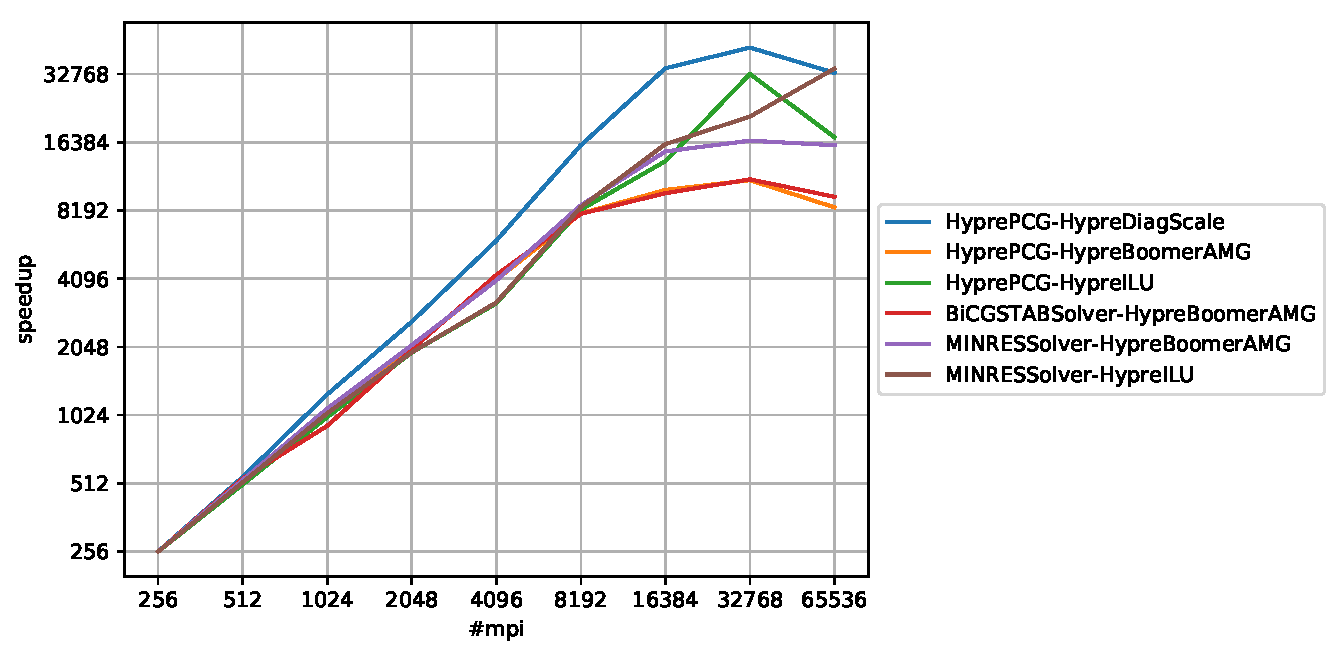
\includegraphics[height=3.6cm]{ver/speedup-r3.pdf}\\[-3mm]
\hspace*{3mm}\scalebox{0.7}{Very good scalability up to \textbf{16k} cores}\\[-1.5mm]
\hspace*{3mm}\scalebox{0.7}{Scalability is superlinear for HyperPCG-HypreDiagScale}
\end{textblock}
\begin{textblock}{.48}(0.58,0.51)
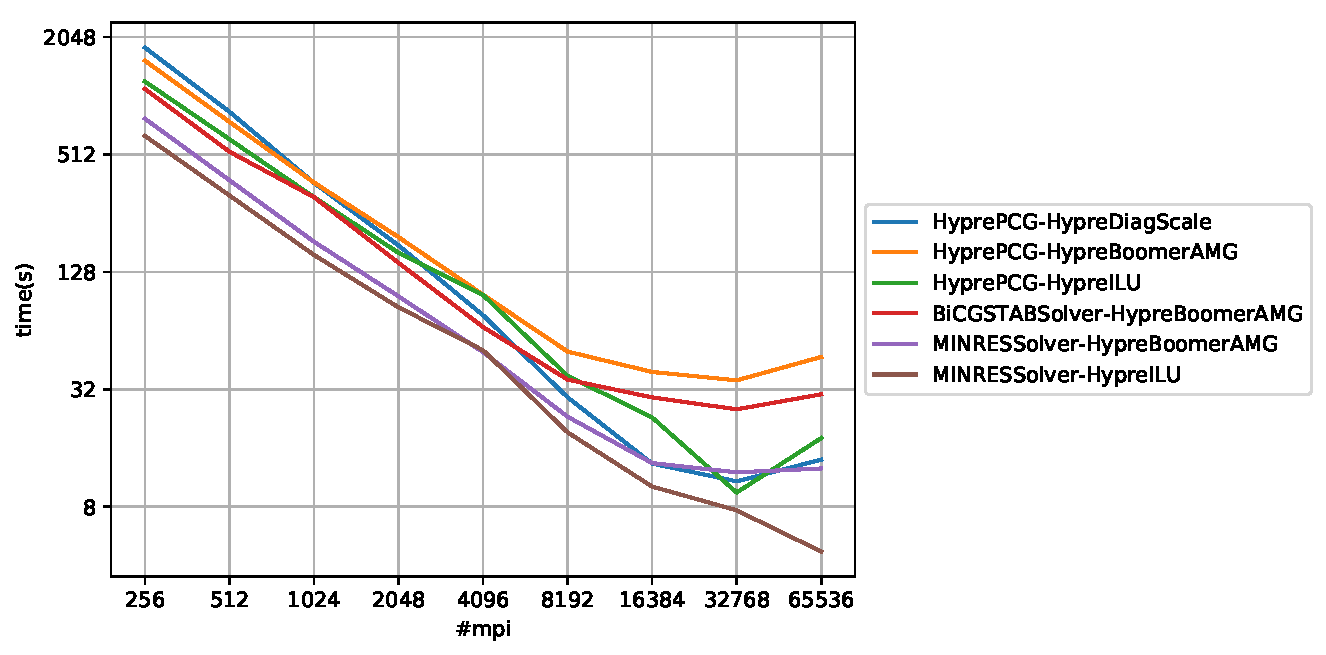
\includegraphics[trim = .1cm .1cm 7.9cm .1cm,clip,height=3.6cm]{ver/timer-r3.pdf}\\[-3mm]
\hspace*{-.5mm}\scalebox{0.7}{\textbf{MINRES+HyperILU} minimizes time to solution}
\end{textblock}
\begin{textblock}{.38}(0.72,0.189)
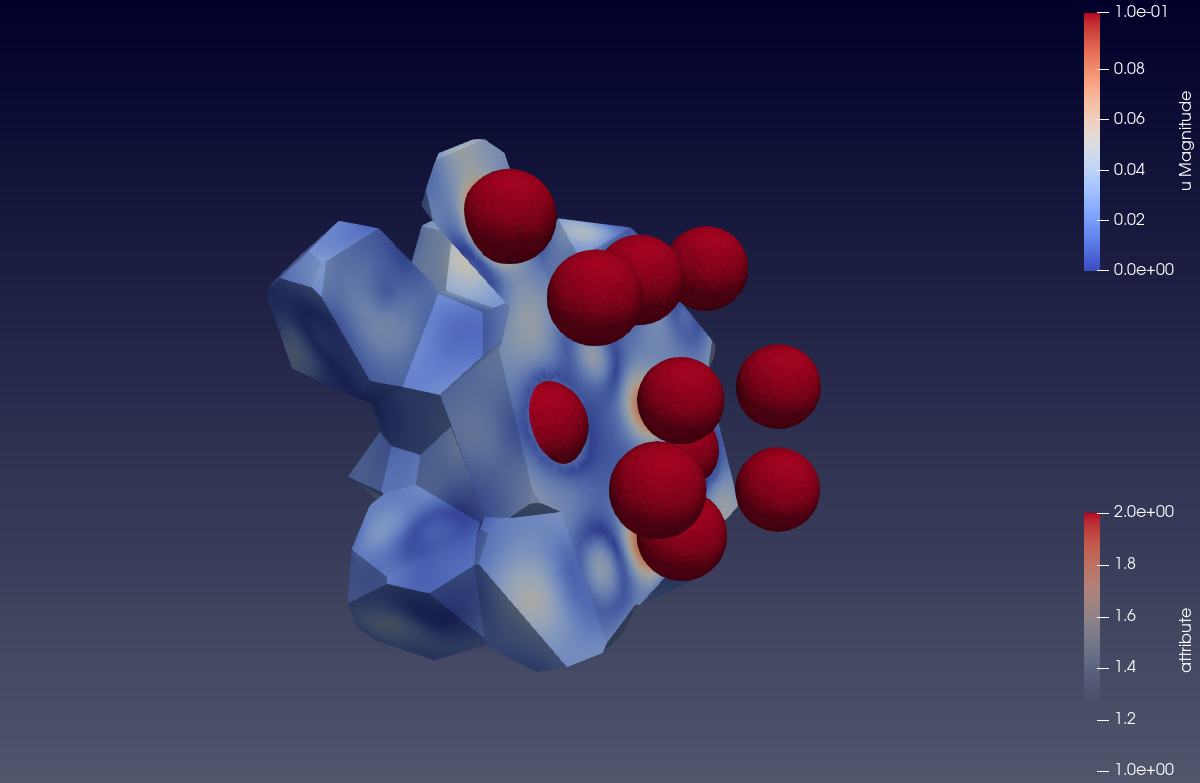
\includegraphics[trim = 2.9cm .1cm 1.cm .1cm,clip,width=3.cm]{ver/vue2.png}\\[-1mm]
\hspace*{3mm}\scalebox{0.7}{3D periodic setting}
\end{textblock}
\end{frame}

\begin{frame}{\scalebox{0.8}{Fuel pellet scale}\\\hspace*{1cm}\scalebox{0.8}{Phase-field modelling}}
  \begin{block}{Modelling fuel pellet fragmentation during reactor start-up}
  \scalebox{0.8}{
    \begin{minipage}{1.28\linewidth}
    \begin{itemize}
      \item Implementing phase-field approach
      \begin{itemize}
      \item Some phase-field models have been previously tested:  AT1, AT2, Lorentz
      \item Micromorphic damage approach used here (David Siedel PhD work - CEA)
      \item Exact treatment of the irreversibility constraint at integration points
      \end{itemize}
      \item $22\ 10^6$ unknowns, \textbf{2500} cores \scalebox{0.8}{(CEA/CCRT computing facility)}
    \end{itemize}
    \end{minipage}}
  \end{block}
  \begin{block}{Numerical results}
    \hspace*{1cm}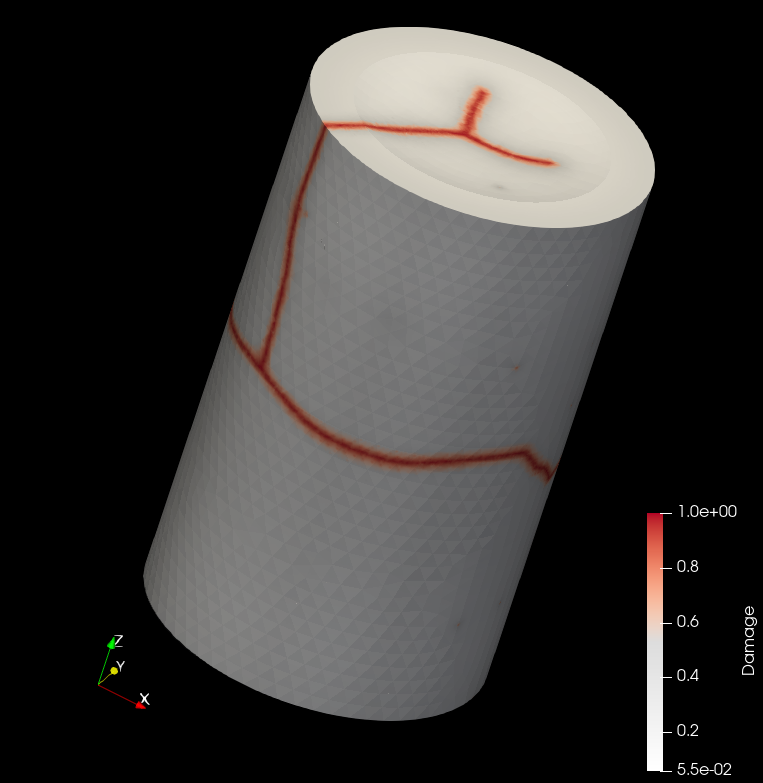
\includegraphics[width=0.3\textwidth]{graphics/damag1.png}
    \hspace*{2cm}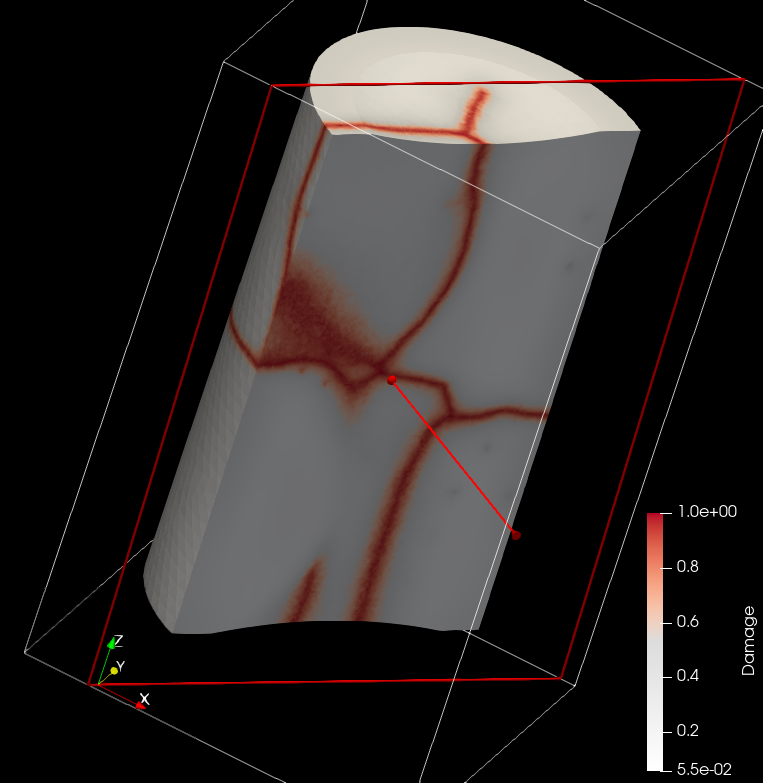
\includegraphics[width=0.3\textwidth]{graphics/damag2.png}
  \end{block}
\end{frame}


\section{Conclusions and perspectives}
\Intercalaire{Conclusions and perspectives}

\begin{frame}{Conclusions and perspectives}
\smallskip
\scalebox{0.9}{
\begin{minipage}{1.1\textwidth}
  \begin{itemize}
    \item What was done ?
    \begin{itemize}
      \item \mmm{} - opensource project thermo-mechanical solver
      \item High level declarative API suitable for
      engineering studies\\\hspace*{1cm} and upcoming integration in {\tt PLEIADES}
      ecosystem
      \begin{itemize}
        \item {\tt MFEM} API still accessible user a lower
        level API
      \end{itemize}
      \item Multi-material support
      \item Ability to handle arbitrary complex finite strain behaviours:
      \begin{itemize}
        \item All behaviours are set at runtime
        (dynamically loaded libraries)
      \end{itemize}
    \end{itemize}
    \vspace*{1mm}
    \item What comes next ?
    \begin{itemize}
      \item Maintain the confidence of industrial partners (EDF, Framatome) on PLEIADES\\
      \hspace*{1cm}keep the funding
      \item Overall robustness of the code, tutorials
      \item Setup extensive continuous integration (github actions + private)
      \item Extension to other physical phenomea (non linear
      heat-transfer, diffusion, non local mechanics). \textit{Should be
        easy} using code generation of behaviour integrators
      \item Adaptative mesh refinements (requires new data
      structures in MGIS) - AMR
      \item Additional boundary conditions, including contact
      with friction
      \item Provide more examples
      \item Checkpoint/restart
      \item Port to GPUs (requires tremendous work on the
      MFront and MGIS side)
      \item Support for partial assembly (if possible ...)
      
    \end{itemize}
  \end{itemize}
    \end{minipage}}
  \begin{textblock}{.26}(0.78,0.12)
%  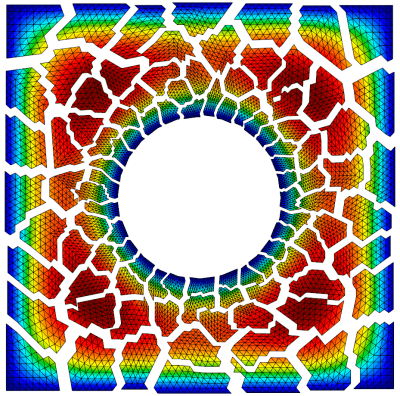
\includegraphics[width=.94\textwidth]{img/ex1p-np100.png}
  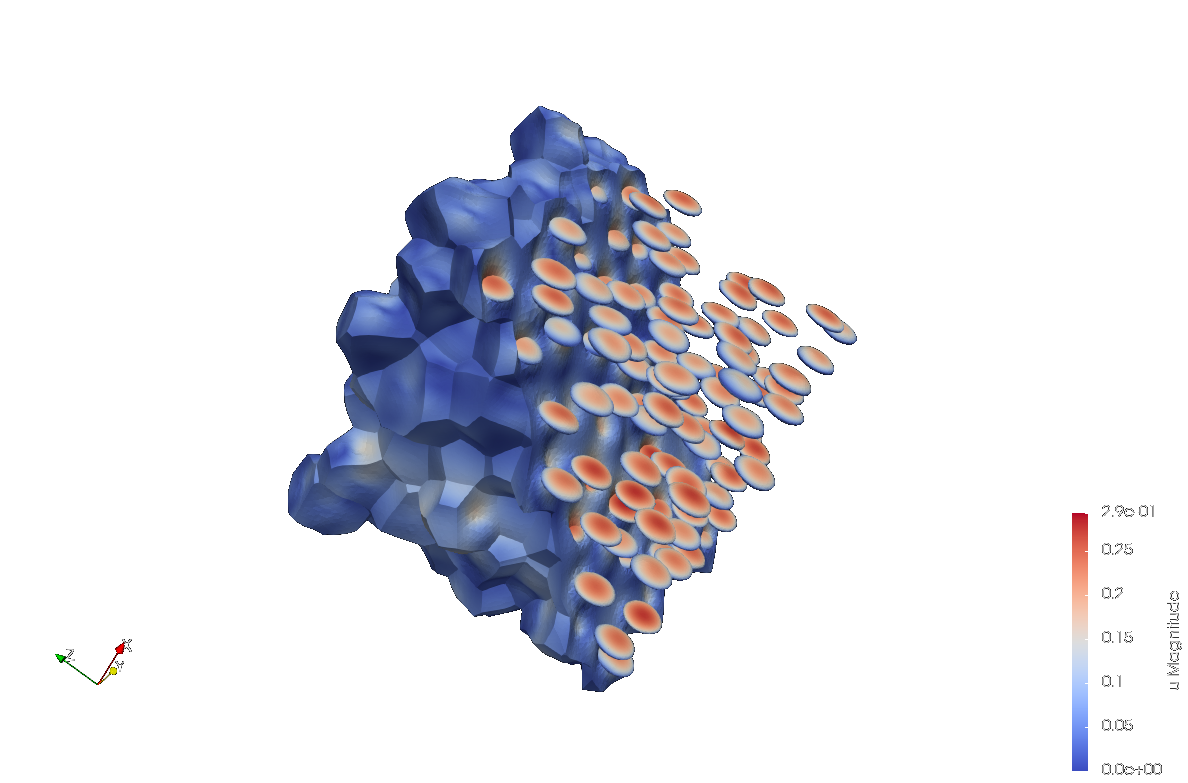
\includegraphics[trim = 8.9cm .1cm 8.cm .1cm,clip,width=.94\textwidth]{ver/222_spheres1.png}
  \end{textblock}
\end{frame}    


\DernierePage{ \vspace*{1.5cm} \hspace*{-1.2cm}
  \scalebox{0.9}{
    \begin{minipage}[h]{0.75\textwidth}
      \begin{center}
        \textcolor{white}{ Thank you for your
          attention.\\ Time for discussion !\\[6mm]
          \small{\url{https://github.com/thelfer/mfem-mgis}}\\
          \small{\url{https://github.com/latug0/mfem-mgis-examples}}\\
          \small{\url{https://github.com/thelfer/MFrontGenericInterfaceSupport}}\\
          \small{\url{https://tfel.sourceforge.net}}\\
          \small{\url{https://www.researchgate.net/project/TFEL-MFront}}\\
        }
      \end{center}
    \end{minipage}
  }
  }
%  \hspace*{-5cm}
%  \vspace{-1.5cm}
%  \scalebox{1}{
%    \begin{minipage}[h]{0.95\textwidth}
%      \textcolor{white}{The development
%        of \texttt{MFront} is supported \\
%        financially by CEA, EDF and Framatome \\
%        in the framework of the \texttt{PLEIADES} project.
%      }
%    \end{minipage}
%  }


%\backupbegin
%\begin{frame}{Non linear resolution\\\hspace*{1cm} in solid mechanics}
%  \begin{itemize}
%     \item    Mechanical equilibrium:
%    find\(\Delta\ensuremath{\mathbb{\uppercase{\vec{u}}}}\) such as: \[
%    \ensuremath{\ensuremath{\mathbb{\uppercase{\vec{R}}}}}{\left(\Delta\ensuremath{\mathbb{\uppercase{\vec{u}}}}\right)}=\ensuremath{\mathbb{\uppercase{\vec{O}}}}\quad\text{
%      avec
%    }\quad\ensuremath{\ensuremath{\mathbb{\uppercase{\vec{R}}}}}{\left(\Delta\ensuremath{\mathbb{\uppercase{\vec{u}}}}\right)}=\ensuremath{\ensuremath{\mathbb{\uppercase{\vec{F}}}}_{i}}{\left(\Delta\ensuremath{\mathbb{\uppercase{\vec{u}}}}\right)}-\ensuremath{\ensuremath{\mathbb{\uppercase{\vec{F}}}}_{e}}
%    \] 
%    \item Resolution using the Newton-Raphson algorithm: \[ 
%    \Delta\ensuremath{\mathbb{\uppercase{\vec{u}}}}^{n+1}=\Delta\ensuremath{\mathbb{\uppercase{\vec{u}}}}^{n}-\ensuremath{\underline{\underline{\mathbf{\mathbb{K}}}}}^{-1}.\ensuremath{\ensuremath{\mathbb{\uppercase{\vec{R}}}}}{\left(\Delta\ensuremath{\mathbb{\uppercase{\vec{u}}}}^{n}\right)}
%    \] 
%        \item  Element contribution to inner forces: \[
%    \ensuremath{\ensuremath{\mathbb{\uppercase{\vec{F}}}}_{i}^{e}}= \sum_{i=1}^{N^{G}} {\left(\ensuremath{\ensuremath{\underline{\mathbf{\sigma}}}}_{t+\Delta\,t}{\left(\Delta\ensuremath{\ensuremath{\underline{\mathbf{\epsilon}}}^{\mathit{to}}}{\left(\vec{\eta}_{i}\right)},\Delta\, t\right)}\colon\ensuremath{\underline{\underline{\mathbf{B}}}}{\left(\vec{\eta}_{i}\right)}\right)}w_{i}
%    \]
%        \item    Element contribution to the stiffness: \[
%    \ensuremath{\underline{\underline{\mathbf{\mathbb{K}}}}}^{e}=\displaystyle\sum_{i=1}^{N^{G}}
%    \mbox{}^{t}\ensuremath{\underline{\underline{\mathbf{B}}}}{\left(\vec{\eta}_{i}\right)}\colon\frac{\displaystyle\partial\,\Delta\ensuremath{\ensuremath{\underline{\mathbf{\sigma}}}}}{\displaystyle\partial\,\Delta\ensuremath{\ensuremath{\underline{\mathbf{\epsilon}}}^{\mathit{to}}}}{\left(\vec{\eta}_{i}\right)}\colon\ensuremath{\underline{\underline{\mathbf{B}}}}{\left(\vec{\eta}_{i}\right)}w_{i}
%    \]
%    \(\scriptsize\frac{\displaystyle\partial\,\Delta\ensuremath{\ensuremath{\underline{\mathbf{\sigma}}}}}{\displaystyle\partial\,\Delta\ensuremath{\ensuremath{\underline{\mathbf{\epsilon}}}^{\mathit{to}}}}\)
%    is the \{\bf consistent tangent operator\}
%  \end{itemize}
%\end{frame}
%\backupend

\end{document}
